\documentclass[12pt,twoside,twoside]{report}

\usepackage{mythesis}      % For most of customized stuff;
\usepackage{graphicx}
\usepackage{setspace}
%\usepackage{subfigure}
\usepackage{subfig}
\usepackage{lingmacros}
\usepackage{tree-dvips}
\usepackage{alltt}
\usepackage{longtable}
\usepackage{amsmath}
\usepackage[english]{babel}
\usepackage{amssymb}
\usepackage{hyperref}


\usepackage[	sorting=none,
				sortcites=true,
		backend=bibtex,
                doi=false,
                isbn=false,
                url=false,
                eprint=false,
                maxbibnames=99,
                style=numeric-comp]
{biblatex}
\bibliography{ref}

\usepackage[T1]{fontenc}

\renewcommand{\v}[1]{\mathbf{#1}}

%%%% Complies with the thesis office regulations

%% Double sided

%\setlength{\evensidemargin}{0.00in}

%% Single sided
%\setlength{\oddsidemargin}{0.50in}
\setlength{\evensidemargin}{0.00in}

%\setlength{\topmargin}{-0.50in}
\setlength{\textwidth}{6.0in}
\setlength{\textheight}{8.85in}
\setlength{\headsep}{0.25in}
\setlength{\parskip}{1em}

%%%% These two lines define spacing for the whole thesis: Magic numbers?
\newcommand{\smallstretch}{0.96}    % footnotes, captions, tables of contents, etc
\newcommand{\textstretch}{1.50}     % The normal text
\newcommand{\foretextstretch}{1.20} % The acknowledgment and outline text
\newcommand{\gparindent}{3ex}       % Three letter wide parindent
\setlength{\parindent}{\gparindent}

\newcommand{\vc}[1]{\mathbf{#1}}
\newcommand{\kpar}{{\vc{k_{||}}}}
\newcommand{\rpar}{{\vc{r_{||}}}}
\newcommand{\slo}{\renewcommand{\baselinestretch}{\smallstretch}\small\footnotesize}
\newcommand{\elo}{\renewcommand{\baselinestretch}{\textstretch}\small\normalsize}

\begin{document}

\pagenumbering{roman}
%%%%%%%%%%%%%%%%%%%%%%%%%%%%%%%%%%%%%%%%%%%%%%%%%%%%%%%%%% TITLEPAGE
%%%% This puts no headings
\pagestyle{empty}
%%%% This is the titlepage
\renewcommand{\baselinestretch}{1.2}\small\normalsize
\vspace*{-0.2in}
\thispagestyle{empty}
\begin{center}
\rule[0pt]{5.6in}{1pt}
\vskip -12pt
\rule[0pt]{5.8in}{3pt}
\vskip 23pt
{\LARGE \sf Classical Nucleation Theory in the
\center{Phase Field Crystal Model}
}
\vskip 13pt
\rule[0pt]{5.8in}{3pt}
\vskip -14pt
\rule[0pt]{5.6in}{1pt}
\end{center}
\vspace{-15pt}
\begin{center}
{\large\sf Paul Jreidini}\\
Centre for the Physics of Materials\\
Department of Physics \\
McGill University \\
Montr\'eal, Qu\'ebec \\
Canada \\
\end{center}
%\vspace{3.5in}
%\vspace{1.50in}
\vfill
%\centerline{\psfig{file=figs/logo.ps}}
\vfill
\begin{center}
A Thesis submitted to the\\
Faculty of Graduate Studies and Research \\
in partial fulfillment of the requirements for the degree of\\
Master of Science\\
\end{center}
\vspace{0.0in}
\begin{center}
{\footnotesize \copyright\ Paul Jreidini, 2017}
\end{center}

\cleardoublepage
%%%%%%%%%%%%%%%%%%%%%%%%%%%%%%%%%%%%%%%%%%%%%%%%%%%     FIRST PART (a)
%%%% Use single spacing for first part.
%%%% Dummy font change required for reset.
\renewcommand{\baselinestretch}{\smallstretch}\small\normalsize
%%%%%%%%%%%%%%%%%%%%%%%%%%%%%%%%%%%%%%%%%%%%%%%%%%%     DEDICATION
%%%% This removes heading
\pagestyle{empty}
%\input{etc/dedication}
%\cleardoublepage
%%%%%%%%%%%%%%%%%%%%%%%%%%%%%%%%%%%%%%%%%%%%%%%%%%%     TABLES OF CONTENTS
%%%% Back to heading in top margin
\pagestyle{headings}
\tableofcontents
\newpage
%%%%%%%%%%%%%%%%%%%%%%%%%%%%%%%%%%%%%%%%%%%%%%%%%%% FIGURES
%%%%
%\listoffigures
%\newpage
%%%% Any table? Uncomment the following line:
%\listoftables
%\newpage
%%%% I prefer to use one page for both
%\listofboth
%\newpage
%%%%%%%%%%%%%%%%%%%%%%%%%%%%%%%%%%%%%%%%%%%%%%%%%%% FIRST PART (b)
%%%% Use slightly larger spacing for remaining of first part.
%%%% We need to reset baselineskip after making each chapter
%%%% entry in order to get a uniform look.
%%%%%%%%%%%%%%%%%%%%%%%%%%%%%%%%%%%%%%%%%%%%%%%%%%%     ABSTRACT
%%%% The English abstract
\renewcommand{\baselinestretch}{\smallstretch}\small\normalsize
\chapter*{\sf Abstract}
\addcontentsline{toc}{chapter}{\protect\hspace{3.5ex}{\sf Abstract}}
\renewcommand{\baselinestretch}{\foretextstretch}\small\normalsize
%   ABSTRACT

An understanding of polycrystalline materials, ranging from alloys to certain ceramics and polymers and beyond, is of great importance for modern society. These materials typically form through the process of nucleation, a thermally activated phase transition. The numerical modeling of this phase transition is problematic for traditional numerical techniques: the commonly used phase field methods' resolution does not extend to the atomic scales at which nucleation takes places, while atomistic methods such as Molecular Dynamics are incapable of scaling to the mesoscale regime where late-stage growth and structure formation takes place following earlier nucleation. As such, there is interest in examining whether the Phase Field Crystal (PFC) model, which attempts to bridge the atomic and mesoscale regimes, is capable of modeling nucleation. In this work, we numerically calculate nucleation rates and incubation times in the PFC model. We show qualitative agreement with classical nucleation theory (CNT), a single-variable stochastic model. We also examine the form and behavior of nuclei at early formation times, finding disagreement with some basic assumptions of CNT. We then argue that a quantitatively correct nucleation theory for the PFC model would require extending CNT to a multi-variable theory.   % the English abstract
\newpage
%%%%%%%%%%%%%%%%%%%%%%%%%%%%%%%%%%%%%%%%%%%%%%%%%%%     RESUME
%%%% The French abstract
\renewcommand{\baselinestretch}{\smallstretch}\small\normalsize
\chapter*{\sf R\'esum\'e}
\addcontentsline{toc}{chapter}{\protect\hspace{3.5ex}{\sf R\'esum\'e}}
\renewcommand{\baselinestretch}{\foretextstretch}\small\normalsize
% abstract, French version

abstract, French version...  % The French 'sommaire'
\newpage
%%%%%%%%%%%%%%%%%%%%%%%%%%%%%%%%%%%%%%%%%%%%%%%%%%%     STATEMENT OF ORIGINALITY
%%%%
\renewcommand{\baselinestretch}{\smallstretch}\small\normalsize
\chapter*{\sf Statement of Originality}
\addcontentsline{toc}{chapter}{\protect\hspace{3.5ex}{\sf Statement of Originality}}
\renewcommand{\baselinestretch}{\foretextstretch}\small\normalsize
The goal of this thesis is numerical comparison between the process of nucleation in the Phase Field Crystal (PFC) model and the predictions of classical nucleation theory (CNT). My contributions towards this goal include:
\begin{itemize}
\item The implementation of code to obtain the nucleation rate and incubation time in the PFC model.
\item The implementation of code to examine the wave mode amplitudes in nuclei during the early stages of nucleation in the PFC model.
\item The implementation of code to approximate the form of the critical nuclei in the PFC model.
\item Deriving equations for the variation of nucleation rate and incubation time following the assumptions of CNT.
\item Applying the implemented code to test the agreement between nucleation in the PFC model and the predictions of CNT.
\end{itemize}












  % The French 'sommaire'
\newpage
%\cleardoublepage
%%%%%%%%%%%%%%%%%%%%%%%%%%%%%%%%%%%%%%%%%%%%%%%%%%%     ACKNOWLEDGMENTS
\renewcommand{\baselinestretch}{\smallstretch}\small\normalsize
\chapter*{\sf Acknowledgments}
\markboth{{\sf Acknowledgments}}{{\sf Acknowledgments}}
\addcontentsline{toc}{chapter}{\protect\hspace{3.5ex}{\sf Acknowledgments}}
\renewcommand{\baselinestretch}{\foretextstretch}\small\normalsize
%   ACKNOWLEDGEMENT

I thank my supervisor, Professor Nikolas Provatas, for his guidance throughout this research project, as well as for his editorial help in preparing this thesis manuscript. I also thank Dr. Nan Wang and Gabriel Kocher for their assistance in understanding both the theory and the numerics behind the PFC model and thermodynamic concepts involved. Finally, I thank the rest of Professor Provatas's research group for their moral support and academic discussions related to this work.
\newpage
%%%%%%%%%%%%%%%%%%%%%%%%%%%%%%%%%%%%%%%%%%%%%%%%%%%     PHYSICAL CONSTANTS AND UNITS
\renewcommand{\baselinestretch}{\smallstretch}\small\normalsize
%\chapter*{\sf Physical Constants and Units}
%\markboth{{\sf Physical Constants and Units}}{{\sf Physical Constants and Units}}
%\renewcommand{\baselinestretch}{\foretextstretch}\small\normalsize
%%	CONSTANTS AND UNITS

\begin{tabular}{lcr}
1 \AA & = & $ 10^{-10} $ m \\
$a_0 $ (Bohr radius) & = & 0.5292 \AA \\
$m_e $ (electron mass) & = & $ 9.1096 \times 10^{-31} $ kg \\
$m_p $ (proton mass) & = & $ 1.6726 \times 10^{-27} $ kg \\
$e$ (electron charge) & = & 1.6 $ \times 10^{-19}  $ C \\
$h$ (Planck's constant) & = & $ 6.626 \times 10^{-34} $ J $\cdot$ s \\
$k_B $ (Boltzmann's constant) & = & $ 1.38 \times 10^{-23} $ K \\
$k_B T $ (at $300 $ K ) & = & $ 0.026 $ eV \\
$c$ (speed of light) & = & $ 2.9979 \times 10^8 $ m/s \\
$G_0 $ (quantum unit of conductance) & = & 7.75 $\times 10^{-5} \Omega^{-1}$ =
$\frac{1}{12.9 \mbox{k}\Omega}$\\
\end{tabular}

\vspace{1.0in}

Atomic units are used throughout this thesis unless otherwise indicated.
In this system of units, $ e = m_e = \hbar = 1 $.

\vspace{1.0cm}

\begin{tabular}{lcccr}
1 unit of Length & = & $ a_0 $  & = & 0.5292 \AA \\
1 unit of Mass & = & $ m_e $  & = & 9.1096 $\times 10^{-31}$ kg \\
1 unit of Charge & = & $ e $  & = & 1.6 $\times 10^{-19}$ C \\
1 unit of Angular momentum & = & $ \hbar $ & = & 1.0546 $ \times 10^{-34} $ J $\cdot$ s \\
1 unit of Energy & = & 1 Hartree & = & 27.2 eV \\
1 unit of Time & = & $ \frac{\hbar}{\mbox{1 Hartree}}$  & = & 2.4189 $ \times 10^{-17}$ s \\
\end{tabular}



%\newpage
%%%%%%%%%%%%%%%%%%%%%%%%%%%%%%%%%%%%%%%%%%%%%%%%%%%%     ABBREVIATIONS
%\renewcommand{\baselinestretch}{\smallstretch}\small\normalsize
% \chapter*{\sf List of Abbreviations}
% \markboth{{\sf List of Abbreviations}}{{\sf List of Abbreviations}}
% \renewcommand{\baselinestretch}{\foretextstretch}\small\normalsize
% %   LIST OF ABBREVIATIONS

\begin{tabular}{cl}
DFT & Density Functional Theory \\
GGA & Generalized Gradient Approximation \\
HF & Hartree-Fock\\
KS & Kohn-Sham \\
LCAO & Linear Combination of Atomic Orbitals \\
L(S)DA & Local (Spin) Density Approximation \\
PS & Pseudopotential \\
SC & Self-Consistent \\
SOC & Spin-Orbit Coupling\\
XC & Exchange-Correlation \\
\end{tabular}

% \newpage
%%%%%%%%%%%%%%%%%%%%%%%%%%%%%%%%%%%%%%%%%%%%%%%%%%%     PADDING
%%%% This puts an empty padding page when required
\pagestyle{empty}
\cleardoublepage
%%%%%%%%%%%%%%%%%%%%%%%%%%%%%%%%%%%%%%%%%%%%%%%%%%%     SECOND PART
\renewcommand{\baselinestretch}{\foretextstretch}\small\normalsize
%%\include{symb}
%%\newpage
%%%% Do you want a separator ?
%\input{etc/title_int}
\cleardoublepage
%%%% Change page numbering to arabic mode
\pagenumbering{arabic}
%%%% Now go to text spacing for second part:
%%%% Dummy font change required for reset.
\renewcommand{\baselinestretch}{\textstretch}\small\normalsize
%%%% Make sure we use headings for second part
\pagestyle{headings}

\chapter{\sf Introduction}\label{ch:intro}

The fields of materials science and engineering are built on a solid understanding of phase transitions, which dictate the microstructure, and hence properties, of most man-made materials.
As the rapid pace of technological progress requires materials with ever more demanding specifications, ranging from stronger steels for taller skyscrapers to semiconductors with finely tuned electronic band structures, constant pressure is placed on these fields to enhance their phase transition models and apply them to the development of novel materials.
The advent of plentiful and inexpensive computing power in the past few decades has greatly benefited this endeavor by allowing the numerical study of phase transition problems that prove intractable otherwise.



In particular, great effort goes into the numerical modeling of polycrystalline materials, which are comprised of numerous microscopic interlocked crystal grains (aka. crystallites) of differing sizes, shapes, orientations, and compositions. These materials include most metals and alloys, as well as some ceramics and polymers, and even a few biological microstructures \cite{jin03}. The morphological and chemical properties of the constituent crystal grains have a direct effect on characteristics of the macroscopic material \cite{granasy_phasefieldnuc,boettinger00}, hence the interest in modeling their formation and evolution. The first step in the grains' formation is the process of nucleation, wherein thermal fluctuations in a progenitor phase stochastically create stable nuclei of a new phase which then proceed to grow. The main difficulty in modeling this process is due to the large range of scales involved: though final grains range in size from a few nanometers to above millimeters depending on the material, the initial nuclei form on atomic lengthscales. Further, some systems are known to exhibit nucleation events simultaneously with large-scale structure evolution, such as in rapidly cooling metal pools formed by laser-beam welding \cite{david03,boettinger00}, and during the so-called columnar to equiaxed transition \cite{kurz01}. While the growth and late evolution of grains are relatively well understood \cite{granasy_02}, there remain open questions concerning how to efficiently and accurately model the initial nucleation stage of formation without impairing the modeling of the much larger scale evolution. 

Various numerical techniques for simulating phase transition processes, including nucleation, have been developed since the 1960s, each best suited to specific types of problems. Among these, traditional phase field methods \cites{hohenberg77,singer08,chaikin_condensed,provatas_PFC} are some of the more widely used in studying microstructure formation. They are well-adapted for simulations on micrometer to millimeter length scales, and on diffusive time scales. These methods consist of multi-field descriptions of phases separated by diffuse interfaces, effectively greatly refined versions of Landau's order parameter theory of phase transition. The fields are spatially continuous, constant within bulk regions, and vary smoothly but rapidly at interfaces. Typically, the fields used can represent order, concentration, and temperature. Phase field methods have been used to simulate assorted material phenomena that include eutectic (multi-species solid mixture) system growth \cite{grant94}, dendritic microstructure evolution \cite{provatas98,kim99}, fracture growth \cite{karma01}, and structure changes in irradiated materials \cite{li17}. However, they face difficulty in modeling physical processes that involve atomistic lengthscales. For example, phenomena that occur on the scale of the width of phase interfaces need special care \cite{karma01_2,elder01,plapp11}, as the phase field models approximate interfaces to be much more diffuse than the typical dozen atom-widths found in real materials, for reasons of computational efficiency. Moreover, effects related to crystalline lattice structure, such as orientation and elastic deformation, do not appear naturally in the basic models, instead requiring more coupled fields to be added \cite{oforiopoku2010,steinbach06,granasy_phasefieldnuc,plapp11} and thus increasing computational and mathematical complexity. As nucleation is a fundamentally atomistic process, phase field models are incapable of modeling it exactly: the processes leading to formation of physically-accurate nuclei can not be resolved at these models' scales. Workarounds to this limitation involve either using unrealistically large thermal fluctuations that force nucleation at the desired time and length scales, or artificially adding already-formed nuclei to the system according to assumed statistics for the material \cite{granasy_phasefieldnuc,granasy_02,plapp11}.

On the other end of the scale spectrum for modeling techniques, atomistic models, such as the Molecular Dynamics (MD) methods \cite{alder59,rapaport_md}, are capable of simulating phenomena difficult to access with phase field methods. These include amorphous solidification of metals \cite{ozgen04,tian08}, properties of atomically-rough interfaces \cite{hoyt01}, and more. Notably, MD methods have had recent success in simulating nucleation and nanoscale grain growth in metals \cite{shibuta15}. These methods typically involve tracking the individual positions and interaction potentials of all the atoms in a system, calculating the dynamics of the resulting N-body problem by numerical integration of Newton's equations of motion. However, the large number of atoms tracked by these methods limits the length and time scales that can reasonably be simulated with current computational speeds to nanometers and nanoseconds respectively. This prevents the scaling of atomistic models for the study of mesoscale structure dynamics, including those that would result from or occur concurrently with nucleation-initiated phase transitions.

Recently, the Phase Field Crystal (PFC) model as first proposed by Elder et al. \cites{elder02,provatas07,emmerich12,humadi13,provatas_PFC} has emerged as a modified phase field method that aims to bridge the gap between atomistic models such as MD and mesoscale models such as traditional phase field methods. Similar to traditional phase field models, the PFC model represents material with a continuous spatial field. However, this field is now periodic in bulk regions, instead of constant. The periodic field acts as an atomic density field, with its peaks denoting the most likely position of the crystal lattice's atoms. Its amplitude represents a phase's order, with the field having zero amplitude in liquid phases and nonzero in solid phases. Figure \ref{fig:phasefield_profile} sketches the profiles of the phase fields in traditional phase field models and the PFC model at a solid-liquid interface, for comparison. In contrast to traditional phase field methods, the PFC method does not have difficulty in describing aspects of the crystal lattice structure, including different grain orientations, grain boundary dynamics \cite{elder08}, lattice defects, and elastoplasticity \cite{elder02,humadi13}. Figure \ref{fig:pfc_example} shows the result of a PFC simulation of solidification for a two-dimensional solid with triangular lattice structure, including some defects that arise in the crystal lattice.

Unlike in `true' atomistic models, atomic movement on vibrational timescales in the PFC model is effectively averaged out, leaving only movement on diffusive timescales. It has been shown \cite{grant08} that applying coarse-graining in time on atomistic simulation methods such as MD methods recovers similar results as the PFC model. Compared to MD methods, PFC is computationally more efficient due to the lack of tracking of individual atoms. This allows studying phenomena appearing at longer time and length scales than MD is reasonably able to simulate \cite{dantzig12}.

\begin{figure}[h]
\centering
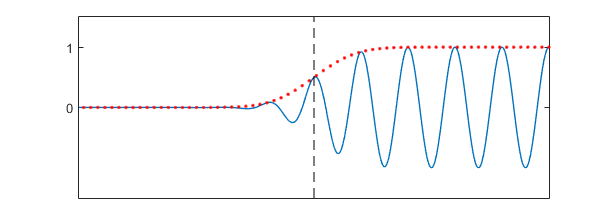
\includegraphics[width=1\textwidth]{fig_pfc/phasefield_profile.png}
\caption{Sketch of profile of phase fields in traditional phase field models (red) and in the PFC model (blue). The x-axis is one dimension of space, and the y-axis is value of the phase field. The vertical dashed line denotes the position of a solid-liquid interface, with the liquid bulk on the left and the solid bulk on the right.}\label{fig:phasefield_profile}
\end{figure}

\begin{figure}[!ht]
\centering
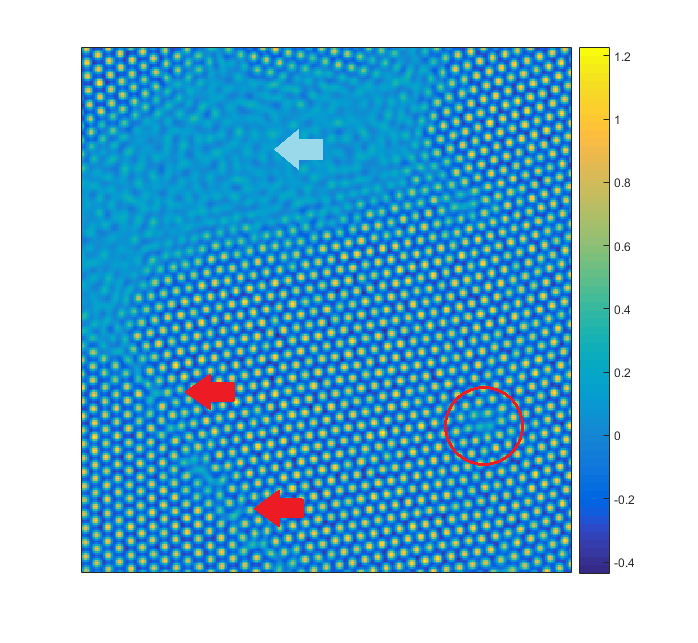
\includegraphics[width=1\textwidth]{fig_pfc/pfc_example_mod2.png}
\caption{Results of a PFC simulation for solidification, showing the phase field in adjacent solid regions with triangular lattices of different orientations, in coexistence with a liquid region. The cyan arrow points to the region of fluctuating liquid, between solid regions. The red arrows point towards a grain boundary between two solid regions of differing orientations. The red circle shows an isolated dislocation defect.}\label{fig:pfc_example}
\end{figure}

For the reasons stated above, the PFC model can be used as an intermediate model between atomistic simulations and the more coarse-grained traditional phase field methods that do not retain the details of the atomic structure. It is thus of interest to examine whether this model can be used to study the process of nucleation without a loss of efficiency nor accuracy. Nucleation is known to occur naturally in the PFC model through the inclusion of thermal fluctuations obeying the fluctuation-dissipation theorem, with the resulting nuclei consisting of few `atoms' as would be expected in a physical system. More specifically, Granasy, Tegze, Toth, and Pusztai have studied aspects of nucleation in the PFC model including nucleation energy barriers, possible amorphous precursor phases, and heteroepitaxy \cite{toth10,toth11}. However, it is yet unclear whether the PFC model can reproduce specifics of the nucleation process predicted by classical nucleation theory, such as the scaling of nucleation rate and incubation time with temperature. The purpose of this thesis is to numerically study the rates of nucleation in the most basic two-dimensional version of the PFC model, for different parameter choices. We aim to compare these rates to those predicted by classical nucleation theory. We also examine the form of stable nuclei in PFC model simulations, as well as their early-time behavior.

The remainder of the thesis is structured as follows. In chapter \ref{ch:pfc}, following a somewhat more detailed description of general phase field models, the PFC model is introduced and its equilibrium and dynamic properties are examined. Chapter \ref{ch:nucleation} introduces the fundamental concepts of classical nucleation theory. The implementation of the numerical tools used to study the material of the previous two chapters is given in chapter \ref{ch:numerics}. Finally, chapter \ref{ch:results} presents a few results of our investigation on nucleation in the PFC model, followed by our concluding summary and thoughts in chapter \ref{ch:conclusion}.

\textit{Note to the reader: All chapter, section, equation, and figure references, as well as citations, are hyperlinked in the digital PDF version of this work, for convenience.}





\chapter{\sf The Phase Field Crystal Model}\label{ch:pfc}

In this chapter, we first cover the general phase field models that preceded the PFC model. Then, the PFC model's free energy functional is derived from a first-principles theory of solidification, and its equilibrium properties are calculated. The phase diagram for the model is obtained. Finally, we define the dynamics of the model, including thermal fluctuations, and determine the conditions for different types of phase transitions to occur.

%%%%%%%%%%%%%%%%%%%%%%%%%%%%%%%%%%%%%%%%%%%%%%%%%%%%%%%%%%%%%%%%%%%%%%%%%%%%%%%%%%%%

\section{General phase field models}\label{sec:pfc_phasefield}

As the PFC model is a subclass of the general phase field models used in the study of phase transitions and interface motion, we give an overview of traditional phase field models. These concepts will be expanded upon in later sections describing the PFC model specifically.

A basic phase field model consists of a scalar field $\phi(\vec{x})$ (the phase field) representing a volume of material being simulated, along with a partial differential equation (PDE) governing the evolution of the phase field through time. The model also defines a free energy for its system in terms of the phase field, and the PDE drives the system towards its energy minima. More advanced models often incorporate multiple coupled fields, such as fields representing position-dependent temperature and solute concentration. Here we only consider single-field models for brevity.

The phase field in the models we consider here acts as an order parameter for the material being simulated: the field is zero in regions where the material is in a disordered phase, and nonzero in regions of ordered phase. For example, a pure material undergoing a phase transition from liquid to crystalline solid can be represented by a phase field corresponding to the density of the material relative to the liquid density, so that $\phi=0$ in the liquid and nonzero in the solid. Another example would be a mean-field Ising spin model where each spin can point in one of two directions, which could be simulated using a phase field model where $\phi$ is proportional to the average magnetization: $\phi=0$ in regions where the spin directions are completely random, and $|\phi|>0$ otherwise, with sign depending on the preferred spin direction. In these examples, the phase field is spatially constant within the bulk of regions with a specific order, and varies smoothly but rapidly at the interface between regions of different order.


For a given phase field model, the value $\phi$ takes in different phases, as well as the type of phase transition that the system undergoes, depends on the choice of local free energy density function $f(\phi,T)$. Here, $T$ is a temperature assumed to be constant over all space. This local free energy density accounts only for the energy in a bulk of constant $\phi$, neglecting interfacial energies between bulks of different $\phi$. Though the function $f$ can in general be an arbitrary function, we use the Landau theory of phase transitions to construct example polynomial forms for $f$ that can be tailored to different types of phase transitions.

Figure \ref{fig:landau_secondorder} plots a local energy density function that exhibits a second order phase transition, characterized by a continuous change of the order parameter as a critical temperature $T_c$ is passed. For $T>T_c$, the energy function has a single minimum at $\phi=0$ corresponding to the disordered phase, while for $T<T_c$ two minima of equal depths exist at nonzero values of $\phi$ corresponding to two ordered phases. The positions of these new minima move continuously from zero as $T$ decreases further from $T_c$. Such an energy function would be used for simulating spinodal decomposition in an Ising spin model with two spin orientations and no external field, or phase separation of two immiscible liquids such as oil and water.

Figure \ref{fig:landau_firstorder} plots a local energy density function that exhibits a first order phase transition, characterized by a discontinuous change of the order parameter as a critical temperature $T_c$ is passed. For $T>T_c$, the energy function's global minimum is at $\phi=0$ corresponding to the disordered phase, while for $T<T_c$ the global minimum has discontinuously moved to a value $\phi>0$ corresponding to an ordered phase. A local minimum exists at $\phi=0$ even for $T<T_c$, indicating the existence of a metastable disordered phase. Such an energy function would be appropriate for simulating solidification of a pure liquid into a solid through the process of nucleation.

\begin{figure}[h]
    \centering
\subfloat[]
{
    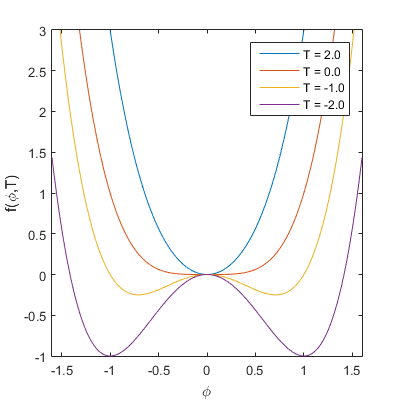
\includegraphics[width=0.5\textwidth]{fig_pfc/landau_secondorder}
    \label{fig:landau_secondorder}
}
\subfloat[]
{
    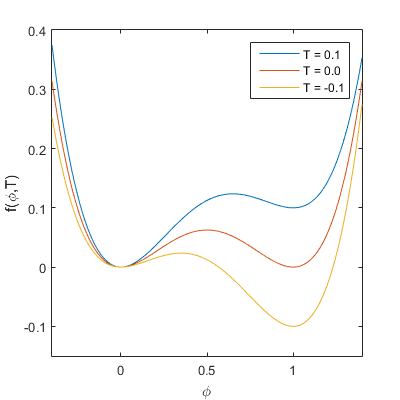
\includegraphics[width=0.5\textwidth]{fig_pfc/landau_firstorder}
    \label{fig:landau_firstorder}
}
    \caption{Plots of local energy density functions that lead to phase transitions at a critical temperature $T_c = 0$. The functions are (a) $f(\phi,T)=T\phi^2+\phi^4$ , (b) $f(\phi,T)=\phi^2(1-\phi)^2 + (3-2\phi)\phi^2T$}\label{fig:landau_functions}
\end{figure}



To evolve a phase field model's system through time, a description of the total energy is needed, including the contribution of interfaces between bulks of constant order parameter. This total energy is defined as a free energy functional $F[\phi]$ of the phase field. Systems consisting of bulk constant-field regions separated by thin interfaces, including the examples mentioned above, can be modeled using the free energy functional
%%
\begin{equation}\label{eq:ginzlandau}
F[\phi,T] = \int \left\{ \frac{1}{2} | W_o \nabla\phi |^2 + f(\phi(\vec{x}),T)  \right\}d\vec{x}
\end{equation}
%%
where the functional integral is over the volume of the system. The first term in the integral corresponds to an energy penalty for interfaces, and vanishes in bulks where the phase field is constant. The parameter $W_o$ determines how large the energy penalty for interfaces is. The term $f(\phi(\vec{x}),T)$ is the local free energy density discussed above. This functional is known as the Ginzburg-Landau free energy \cite{huang_statmech}.

The time-evolution PDE for a phase field model is chosen depending on whether the total phase field (i.e. the integral of the field over all space) is conserved. For example, the total phase field in an Ising model is not necessarily conserved, as there can be an arbitrary number of spins flipping to a new direction. Conversely, the spinodal decomposition of a mixture of immiscible liquids requires a conserved total phase field, assuming the total volume of each component liquid does not change. Nucleation of a solid from a pure liquid would also have conserved total field, due to conservation of mass. As our goal is to describe nucleation, we give here the PDE for a phase field model with conserved total field, which is
%%
\begin{equation}\label{eq:modelB}
\frac{\partial\phi}{\partial t}=M\nabla^2\frac{\delta F}{\delta \phi}
\end{equation}
%%
where $\frac{\delta F}{\delta \phi}$ is the functional derivative of $F[\phi]$, and $M$ is a solute mobility parameter. This PDE is known as the Cahn-Hilliard equation, or as Model B in condensed matter physics circles \cite{hohenberg77}. While we have introduced it in the context of traditional phase field methods, it will also be used in a later section for the PFC model. Figure \ref{fig:phasefield_spinodal} shows a system undergoing spinodal decomposition, simulated using the PDE of equation \ref{eq:modelB}, with the function $f(\phi,T)$ shown in figure \ref{fig:landau_secondorder} and with $T=-0.1$, $W_o=0.2$, and $M=1$.

\begin{figure}[!ht]
    \centering
\begin{tabular}{cccc}
\subfloat[]
{
    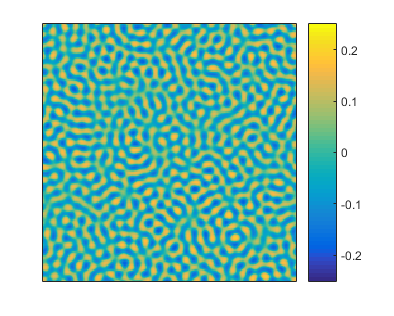
\includegraphics[width=0.5\textwidth]{fig_pfc/spinodal_5}
}
&\subfloat[]
{
    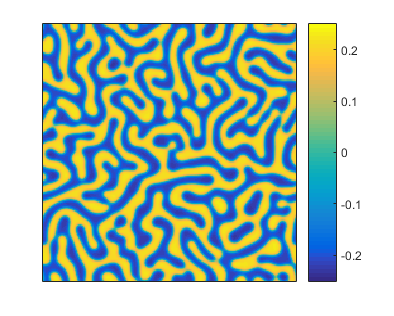
\includegraphics[width=0.5\textwidth]{fig_pfc/spinodal_10}
}\\
\subfloat[]
{
    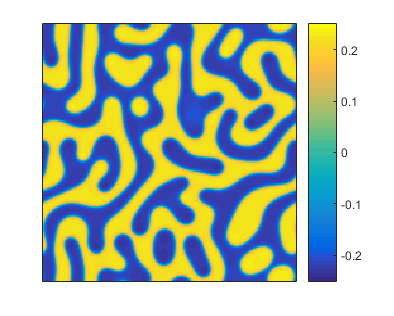
\includegraphics[width=0.5\textwidth]{fig_pfc/spinodal_40}
}
&\subfloat[]
{
    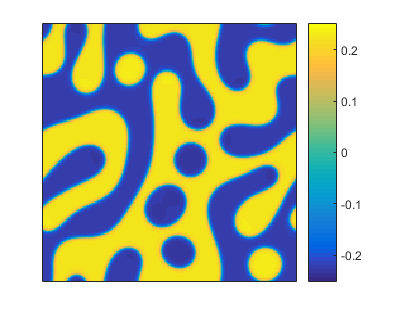
\includegraphics[width=0.5\textwidth]{fig_pfc/spinodal_200}
}
\end{tabular}
    \caption{Simulation of spinodal decomposition with a conserved total phase field, starting from a single disordered phase. The colors represent the phase field $\phi$. (a) to (d) are arranged in order of time, with initial disordered-only state not shown.}\label{fig:phasefield_spinodal}
\end{figure}

%%%%%%%%%%%%%%%%%%%%%%%%%%%%%%%%%%%%%%%%%%%%%%%%%%%%%%%%%%%%%%%%%%%%%%%%%%%%%%%%%%%%

\section{Deriving a free energy functional for PFC}\label{sec:pfc_deriv}

Instead of having a free energy functional that is minimized by bulk regions of constant phase field separated by thin interfaces, the PFC model's energy functional is minimized by a periodic phase field with a constant amplitude in the solid bulk and zero amplitude in the liquid bulk. The PFC model was originally defined as a phenomenological model built to reproduce certain atomic-scale structures and behaviors using a periodic phase field, following earlier work by Swift and Hohenberg \cite{hohenberg77-2} that derived a PDE exhibiting periodic pattern formation in convective systems. However, here we will instead derive the PFC model's free energy functional from classical density functional theory (CDFT) of solidification, and later obtain the PFC model's time-evolution PDE from this functional. The derivation presented below is for a two-dimensional system consisting of a single atomic specie capable of existing in a liquid phase and a solid phase, where the solid phase exhibits a triangular lattice structure. This derivation can be extended to allow a system in three dimensions, with more than one atomic specie, and with more complicated lattice structures \cites{provatas07,provatas_PFC,greenwood10,greenwood11,greenwood11_2}.

The CDFT used in the derivation, first proposed by Ramakrishnan and Yussouff \cite{ramakrishnan79}, provides as a starting point a Helmholtz free energy functional $\mathcal{F}[\rho]$ where $\rho(\vec{r})$ is the local number density of atoms in the system at position $\vec{r}$. Ramakrishnan and Yussouff obtain this free energy by expanding the full energy functional close to a reference liquid state in coexistence with a solid. Taking the reference liquid's density to be $\rho_o$ and defining $\delta\rho(\vec{r})=\rho(\vec{r})-\rho_o$, they show that
%%
\begin{equation}\label{eq:ramakF}
\frac{\mathcal{F}}{k_B T}= \int \left\{ \rho \ln\left(\frac{\rho}{\rho_o}\right)-\delta\rho \right\}d\vec{r} - \sum_{n=2}^{\infty} \frac{1}{n!} \int \prod_{i=1}^{n} d\vec{r}_i \delta\rho(\vec{r}_i)C_n(\vec{r}_1,\vec{r}_2,\vec{r}_3, ... ,\vec{r}_n)
\end{equation}
%%
where the integrals are over the volume of the system. $T$ is the temperature of the system, assumed to be constant through space, and $k_B$ is the Boltzmann constant. The functions $C_n$ are the $n$-point direct correlation functions of the liquid phase. The first approximation in this derivation is to truncate the integral series up to the two-point correlation function $C_2$. As the liquid phase is assumed to be isotropic, this correlation function can be simplified: $C_2(\vec{r}_1,\vec{r}_2)=C(|\vec{r}_1-\vec{r}_2|)$, where we have dropped the subscript for convenience. The truncated functional is then
%%
\begin{equation}\label{eq:ramakF_truncated}
\frac{\mathcal{F}}{k_B T}= \int \left\{ \rho \ln\left(\frac{\rho}{\rho_o}\right)-\delta\rho \right\}d\vec{r} - \frac{1}{2}\iint C(|\vec{r}_1-\vec{r}_2|)d\vec{r}_1 \delta\rho(\vec{r}_1)d\vec{r}_2 \delta\rho(\vec{r}_2)
\end{equation}
%%

\begin{figure}[h]
\centering
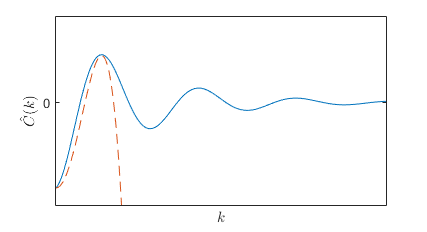
\includegraphics[width=0.8\textwidth]{fig_pfc/fourierCorrelation.png}
\caption{Sketch of the Fourier transform of the two-point direct correlation function. The solid curve is the full shape, the dashed curve is the approximated shape that includes only the first peak.}\label{fig:correlation_fourier}
\end{figure}

The next approximation is for the form of the correlation function $C$. In general, the Fourier transform $\hat{C}(k)$ of the two-point correlation function of a liquid formed of atoms that interact by the Lennard-Jones potential exhibits a rapidly decaying periodic shape \cite{mandel70}, due to the lack of long-range order. Figure \ref{fig:correlation_fourier} sketches the shape of such a function. We fit a polynomial function in Fourier space that matches only the first peak of the full function, approximating
%%
\begin{equation}\label{eq:correlationFourier}
\hat{C}(k) \approx -\hat{C}_0+\hat{C}_2 k^2 - \hat{C}_4 k^4
\end{equation}
%%
where $\hat{C}_0$, $\hat{C}_2$, and $\hat{C}_4$ are positive constants chosen so that the peaks match in position and height. The position of the peak in Fourier space determines the fundamental wavelength-scale of the resulting crystalline solid's reciprocal lattice. As there is only a single wavelength-scale, this approximate one-peak correlation function leads to a triangular lattice structure, the simplest two-dimensional Bravais lattice. A different choice for the correlation function can lead to more complex lattice symmetries \cite{greenwood10,greenwood11}. By calculating the position of the peak in Fourier space, we can obtain the real-space lattice constant $\alpha$ of the solid phase in terms of the constants appearing in equation \ref{eq:correlationFourier}, $\alpha = \sqrt[]{{2 \hat{C}_4}/{\hat{C}_2}}$, where we dropped a factor of $4\pi/\,\sqrt[]{3}$ for convenience. Taking the inverse Fourier transform of equation \ref{eq:correlationFourier} returns the correlation to real space giving
%%
\begin{equation}\label{eq:correlationReal}
C(|\vec{r}_1-\vec{r}_2|) \approx (-\hat{C}_0-\hat{C}_2 \nabla^2 - \hat{C}_4 \nabla^4)\delta(|\vec{r}_1-\vec{r}_2|)
\end{equation}
%%
where $\delta$ is the Dirac delta function.

Next, we define the dimensionless density field $n(\vec{r})=(\rho(\vec{r})-\rho_o)/\rho_o$ which will act as the phase field in our final derived energy functional. We also rescale the spatial variable by the lattice constant, $\vec{x} = \vec{r}/\alpha$. Plugging $n$ into equation \ref{eq:ramakF_truncated}, expanding the nonlinear term in the first integral to fourth order in $n$, and applying one integration on the correlation function obtained in equation \ref{eq:correlationReal} gives
%%
\begin{multline}\label{eq:derivedFunctional}
\frac{\mathcal{F}}{k_B T \rho_o \alpha^2}= \int d\vec{x}  \left\{2n + \frac{n^2}{2} - \frac{n^3}{6}+\frac{n^4}{12}\right\} \\ +\int d\vec{x}\left\{  -\frac{(n+1)^2}{2}(1-B^l+B^x)+ \frac{(n+1)}{2}B^x(2\nabla^2+\nabla^4)n \right\}
\end{multline}
%%
where we have defined $B^l=1+\rho_o \hat{C}_0$ and $B^x=\rho_o \hat{C}_2^2/4\hat{C}_4$. The final approximation of this derivation is to drop the terms in the integral of less than second order in $n$. This is done because constant terms and terms of first order in $n$ can only add a constant to the free energy functional: As $n$ is assumed to be a periodic function, integrating it over a volume much larger than the lattice constant $\alpha$ averages to a constant. We thus obtain the dimensionless free energy functional $F[n]$ used for the PFC model in all following sections,
%%
\begin{equation}\label{eq:PFC_energyFunctional}
F=\frac{\mathcal{F}}{k_B T \rho_o \alpha^2}= \int d\vec{x} \left\{ \frac{n^2}{2}B^l +\frac{n}{2}B^x(2\nabla^2+\nabla^4)n -t \frac{n^3}{3} + v \frac{n^4}{4}\right\}
\end{equation}
%%
where we have defined $t=1/2$ and $v=1/3$. The reason for these new parameters $t$ and $v$ is phenomenological: As the above derivation involved many crude approximations, it is expected that the resulting free energy functional might need to be tweaked under some circumstances to fit specific requirements. These parameters provide some degrees of freedom allowing such tweaking.

Define $\Delta B = B^l - B^x$. This quantity acts as the effective temperature of the derived PFC model. Returning to the definitions of $B^l$ and $B^x$ and to equation \ref{eq:correlationFourier}, we find that $\Delta B = 1 + \rho_o (\hat{C}_0-\hat{C}_2^2/\hat{C}_4)=1-\rho_o \hat{C}_m$ where $\hat{C}_m$ is the global maximum of the Fourier transformed two-point correlation function. If we fix $\rho_o$ while decreasing $\Delta B$, the peak of the correlation function increases, and vice versa. A higher peak in the correlation function $\hat{C}(k)$ indicates increased preference for the atoms to arrange themselves according to the solid phase's reciprocal lattice structure. Thus, decreasing $\Delta B$ is expected to trigger phase transition from liquid to solid, as will be seen in the following sections.




%%%%%%%%%%%%%%%%%%%%%%%%%%%%%%%%%%%%%%%%%%%%%%%%%%%%%%%%%%%%%%%%%%%%%%%%%%%%%%%%%%%%
\section{The one mode approximation}\label{sec:pfc_1mode}

As discussed in section \ref{sec:pfc_phasefield}, the phases and phase transitions in traditional phase field methods are determined by the local free energy density, a function of the order parameter. While the PFC model's dimensionless density field $n(\vec{x})$ does not act like a true order parameter in the way seen in that section, we can recover a pseudo-order parameter proportional to the amplitude of the periodic field $n$ by exploiting the periodicity to write a `one mode approximation' for $n$. This approximation then allows us to calculate the amplitude of the periodic field in the solid phase, as well as the dimensionless lattice constant of the solid phase.

Consider a system consisting of a single crystalline solid phase with no defects and a unique orientation. As the system is periodic, we can use reciprocal lattice theory to write
%%
\begin{equation}\label{eq:reciprocalLattice}
n(\vec{x}) = n_o + \sum_{\vec{G}} \phi_{\vec{G}} \cos(\vec{G} \cdot \vec{x})
\end{equation}
%%
where $n_o$ is the average of $n$ over the whole system, $\vec{G}$ are the reciprocal lattice vectors, and $\phi_{\vec{G}}$ are the corresponding amplitudes. The reciprocal lattice vectors can be expressed in two dimensions as $\vec{G}=\upsilon_1 \vec{q}_1+\upsilon_2 \vec{q}_2$ where $\vec{q}_i$ are the principle lattice vectors and $\upsilon_i$ are integers. For a triangular lattice in two dimensions, the principle reciprocal lattice vectors can be chosen as
%%
\begin{equation}\label{eq:principalRecVec}
\vec{q}_1 = -\frac{2}{\sqrt[]{3}}\cdot\frac{2\pi}{a}\left(\frac{\sqrt[]{3}}{2}\hat{x}+\frac{1}{2}\hat{y}\right), \qquad \vec{q}_2 = \frac{2}{\sqrt[]{3}}\cdot\frac{2\pi}{a}\hat{y}
\end{equation}
%%
where $a$ is the real-space lattice constant in dimensionless units, not to be confused with the dimensional lattice constant $\alpha$ used in the previous section.

The one mode approximation involves keeping only the terms in equation \ref{eq:reciprocalLattice} corresponding to the lowest order reciprocal lattice vectors. For a triangular lattice, these are the reciprocal lattice vectors for which $(\upsilon_1,\upsilon_2)\in \{(1,0),(0,1),(1,1)\}$. We then take the amplitudes $\phi_{\vec{G}}$ to all be equal, $\phi_{\vec{G}}=\phi/2$ for some parameter $\phi$. Applying the one mode approximation to equation \ref{eq:reciprocalLattice} and simplifying gives
%%
\begin{equation}\label{eq:oneMode}
n(x,y) = n_o + \phi\left(\frac{1}{2}\cos\left(\frac{4\pi}{\sqrt[]{3} a}y\right) - \cos\left(\frac{2\pi}{a}x\right)\cos\left(\frac{2\pi}{\sqrt[]{3} a}y\right) \right)
\end{equation}
%%

We then calculate the total free energy of the system by plugging equation \ref{eq:oneMode} into the free energy functional given by equation \ref{eq:PFC_energyFunctional}. Evaluating the resulting integral and minimizing the total free energy with respect to the lattice constant $a$ \cite{provatas_PFC}, we obtain that the energy is minimized for $a=4\pi/\,\sqrt[]{3}$ and is given in terms of the parameters $\phi$, $n_o$, $B^l$, and $B^x$ as
%%
\begin{multline}\label{eq:freeEnergy_minimized}
F(\phi, n_o, B^l, B^x) = B^l\frac{n_o^2}{2} -t\frac{n_o^3}{3}+v\frac{n_o^4}{4} \\ +\frac{3}{16}(\Delta B -n_o(2t-3vn_o))\phi^2 -\frac{1}{16}(t-3vn_o)\phi^3 + \frac{45v}{512}\phi^4
\end{multline}
%%

We find the locations of the minima of this energy function with respect to $\phi$ to be
%%
\begin{equation}\label{eq:freeEnergy_minima}
\phi_l=0 , \qquad \phi_s = \frac{4}{15v}\left(t-3 v n_o +\sqrt[]{t^2-15v\Delta B +12n_o v(2t-3vn_o)} \right)
\end{equation}
%%

The free energy function given in equation \ref{eq:freeEnergy_minimized} is analogous to the local free energy density function $f$ discussed in section \ref{sec:pfc_phasefield}: the parameter $\phi$ is the equivalent of the order parameters of traditional phase field models, while $\Delta B$ acts as an effective temperature. Figure \ref{fig:deltaB_wells} plots the free energy given by equation \ref{eq:freeEnergy_minimized} as a function of $\phi$ for different $\Delta B$, with fixed $n_o=0$. We observe the form of a free energy function that leads to a first-order transition between solid and liquid phases as $\Delta B$ decreases, with the minimum at $\phi=\phi_l=0$ corresponding to the liquid where the amplitude of the PFC model's periodic phase field $n$ is zero, and the minimum at $\phi=\phi_s>0$ corresponding to the solid where the amplitude is nonzero. Thus, by plugging equation \ref{eq:freeEnergy_minima} into equation \ref{eq:oneMode}, we predict that the value of the density field $n$ in the solid oscillates between $n_o+1.5\phi_s$ and $n_o-1.5\phi_s$.


\begin{figure}[h]
\centering
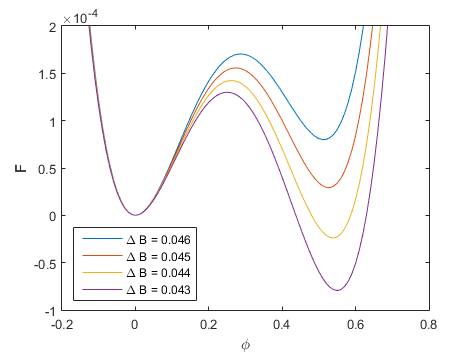
\includegraphics[width=0.8\textwidth]{fig_pfc/deltaBwells.png}
\caption{Free energy function for a single isolated phase, obtained through the one-mode approximation.}\label{fig:deltaB_wells}
\end{figure}




%%%%%%%%%%%%%%%%%%%%%%%%%%%%%%%%%%%%%%%%%%%%%%%%%%%%%%%%%%%%%%%%%%%%%%%%%%%%%%%%%%%%
\section{The PFC model's phase diagram}\label{sec:pfc_phasediag}


While we have approximated the free energy of a single isolated phase (equation \ref{eq:freeEnergy_minimized}) and described how it predicts a first-order phase transition as $\Delta B$ is varied, an actual simulated system can contain both liquid and solid phases in coexistence. Further, most physical materials are known to also transition from liquid to solid as the density is increased at fixed temperature. We will construct a phase diagram for our PFC model that depends on both the effective temperature $\Delta B$ and the average dimensionless density $n_o$, and includes areas of coexisting liquid and solid phases.

The usual method for determining the densities at which two phases coexist is to use the common tangent construction \cite{lupis_materials}. We first calculate the free energy curves of the solid and liquid phases in terms of $B^l$, $B^x$, and $n_o$. Setting $\phi=\phi_s$ in equation \ref{eq:freeEnergy_minimized} gives the free energy function $F_s$ for the solid phase in our model (not shown for brevity), and the free energy function $F_l$ for the liquid phase is obtained by setting $\phi=0$ in that equation, giving
%%
\begin{equation}\label{eq:freeEnergy_minimized_liquid}
F_l = B^l\frac{n_o^2}{2} -t\frac{n_o^3}{3}+v\frac{n_o^4}{4}
\end{equation}
%%

Then, fixing $B^l$ and $B^x$ to fix the effective temperature $\Delta B$, the free energies of the two coexisting phases are plotted as a function of average density $n_o$, and the common tangent to these two curves is found. Figure \ref{fig:commonTangent} plots the free energies of the liquid and solid phases as a function of $n_o$, at a fixed $\Delta B$, including the common tangent construction. Let $n_s$ and $n_l$ be the densities at which the common tangent intersects the energy curves of the solid and liquid phases respectively. For any density $n_o$ satisfying $n_l<n_o<n_s$, the system consists at equilibrium of coexisting phases, with average density $n_l$ for the liquid phase and $n_s$ for the solid phase. For densities where $n_o<n_l$ or $n_o>n_s$, the system at equilibrium consists fully of liquid or solid phase respectively. By repeating this construction for different $\Delta B$, we obtain the system's phase diagram as a function of $n_o$ and $\Delta B$. Figure \ref{fig:pfc_phasediag} displays part of the resulting phase diagram, including the `instability curve' defined later in section \ref{sec:pfc_phasetrans}.

\begin{figure}[h]
\centering
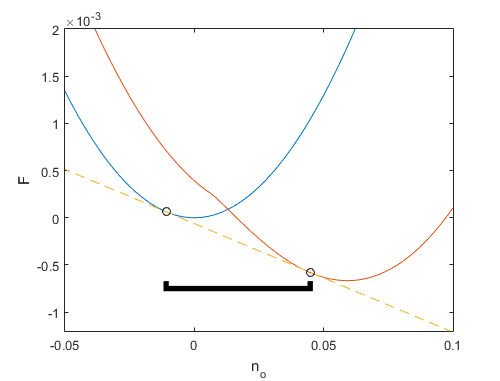
\includegraphics[width=0.8\textwidth]{fig_pfc/commonTangentMod.png}
\caption{The common tangent construction for $B^x=1$ and $B^l=1.055$. The energy function $F_l$ of the liquid phase is in blue, the energy function $F_s$ of the solid phase in red. The yellow line is the common tangent. The black circles are the points of intersection at densities $n_l$ (left) and $n_s$ (right). The black bar denotes the range of densities where the two phases coexist at equilibrium.  }\label{fig:commonTangent}
\end{figure}

\begin{figure}[h]
\centering
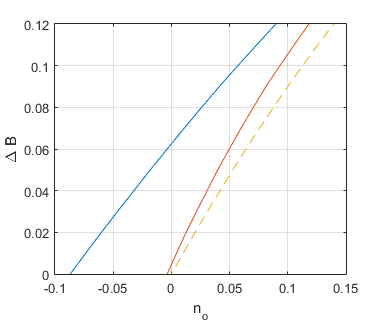
\includegraphics[width=0.8\textwidth]{fig_pfc/phaseDiagSpin.png}
\caption{Phase diagram of the PFC model, for $B^x=1$ fixed. The blue (red) curve is the locus of points $n_l$ ($n_s$) found through the common tangent construction, known as the `liquidus' (`solidus'). The yellow curve is the `instability curve'.}\label{fig:pfc_phasediag}
\end{figure}

%%%%%%%%%%%%%%%%%%%%%%%%%%%%%%%%%%%%%%%%%%%%%%%%%%%%%%%%%%%%%%%%%%%%%%%%%%%%%%%%%%%%
\section{The PFC model's dynamics}\label{sec:pfc_dynamics}

As the phase field of the PFC model represents an atomic density, the field must be conserved as the system is evolved. The time-evolution PDE of the model is thus the same as that of the traditional phase field Model B shown in equation \ref{eq:modelB}. We start with the PDE for the time-evolution of the dimensionful density $\rho(\vec{r})$ in terms of the free energy functional $\mathcal{F}$ of equation \ref{eq:ramakF_truncated},
%%
\begin{equation}\label{eq:pfc_dynamics_dimensionful}
\frac{\partial \rho}{\partial t} = M \nabla^2 \left(\frac{\delta \mathcal{F}}{\delta \rho}\right) + \nabla \cdot \vec\zeta
\end{equation}
%%
where $M$ is a solute mobility parameter and $\nabla \cdot \vec\zeta$ is a noise term representing thermal fluctuations that conserve the total field. $\vec\zeta=(\zeta_x(\vec{r},t),\zeta_y(\vec{r},t))$ is a two-component random vector field uncorrelated with itself in space and time, and satisfying the fluctuation-dissipation relation \cite{chaikin_condensed,sancho_noise}, expressed as
%%
\begin{equation}\label{eq:pfc_noise_dimensionful}
\langle \zeta_i(\vec{r},t),\zeta_j(\vec{r}\,',t') \rangle = -2 k_B T M \delta(\vec{r}-\vec{r}\,')\delta(t-t')\delta_{ij}
\end{equation}
%%
where $T$ is the temperature, $k_B$ is the Boltzmann constant, $\delta(\cdot)$ is the Dirac delta function, and $\delta_{ij}$ is the Kronecker delta function. Equation \ref{eq:pfc_noise_dimensionful} is to be interpreted as specifying that each $\zeta_i$ is a random variable uncorrelated with itself and follows a Gaussian distribution with standard deviation $\sigma = \sqrt[]{2k_B T M}$.

To obtain the time-evolution PDE corresponding to our dimensionless free energy functional $F=\mathcal{F}/k_B T \rho_o \alpha^2$ of equation \ref{eq:PFC_energyFunctional}, we again set $n=(\rho-\rho_o)/\rho_o$ and $\vec{x}=\vec{r}/\alpha$, giving
%%
\begin{equation}\label{eq:pfc_dynamics_dimensionless}
\frac{\partial n}{\partial t} = \Gamma \nabla^2 \left(\frac{\delta F}{\delta n}\right) + \nabla \cdot \vec\xi
\end{equation}
%%
where $\Gamma = k_B T M/\rho_o $ and the dimensionless noise term satisfies
%%
\begin{equation}\label{eq:pfc_noise_dimensionless}
\langle \xi_i(\vec{x},t),\xi_j(\vec{x}\,',t') \rangle = - N_a^2 \delta(\vec{x}-\vec{x}\,')\delta(t-t')\delta_{ij}
\end{equation}
%%
for $N_a^2=2\Gamma/\rho_o \alpha^2$ \cite{kocher16}. Evaluating the functional derivative in equation \ref{eq:pfc_dynamics_dimensionless} gives the time-evolution PDE for the dimensionless density $n(\vec{x})$, written as
%%
\begin{equation}\label{eq:pfc_dynamics_dimensionless_final}
\frac{\partial n}{\partial t} = \Gamma \nabla^2 \left[(B^l +B^x (2\nabla^2+\nabla^4))n -tn^2+vn^3\right] + \nabla \cdot \vec\xi
\end{equation}
%%

What remains is to specify the value of the dimensionless noise standard deviation, $N_a$. While one could attempt to match it to a specific real material's values of $\rho_o$ and $\alpha$, it has been shown by Kocher, Ofori-Opoku, and Provatas \cite{kocher16} that $N_a$ must be chosen as a function of the PFC model's $B^l$ and $B^x$ parameters to ensure proper behavior of capillary fluctuations. These authors also show that a cutoff must be applied to the noise's spectrum: noise modes with wavenumber $k>2\pi/a$ in Fourier space must be set to zero, where $a$ is the dimensionless lattice constant. This cutoff can be understood as eliminating unphysical fluctuations on scales smaller than the lattice separation, as these fluctuations would have already been accounted for in obtaining the CDFT used in section \ref{sec:pfc_deriv} to derive the PFC model's free energy functional. It can also be understood from a numerical perspective \cite{plapp11}: not implementing such a cutoff causes the atomic-scale dynamics of the simulated model to strongly depend on the discretization scheme used, due to more noise modes being available for a finer grid discretization.

Though we have scaled out the dimensional temperature from equation \ref{eq:pfc_noise_dimensionless}, we require that the steady probability distribution of states of our system continue obeying the Boltzmann distribution. To ensure this, the fluctuation-dissipation theorem must again be obeyed \cite{sancho_noise} by defining a fluctuation temperature $T_{r}$ through $N_a^2\approx 2\Gamma T_{r}$. The relation is only approximate due to the cutoff applied to the noise's Fourier modes, and the Boltzmann constant $k_B$ is assumed to be included in $T_r$. In this work, we assume that $T_{r}$ is used in calculating values related to the fluctuation-driven dynamics of the system, such as the Boltzmann factor $\exp(-E/T_r)$ that gives the probability of a state of energy $E$ relative to the probability of a state of zero energy. This fluctuation temperature should not be confused with either the dimensional $T$ that was scaled out of the PFC model's equations, or $\Delta B$ which is normally considered the model's effective temperature due to its previously-detailed role in determining the phase diagram. While $\Delta B$ and $T_{r}$ are effectively coupled by following the recommended values of $N_a$ from \cite{kocher16}, care should be taken when using these separate values in equations that require a temperature value or dependence. 

%It should be noted that the choice of noise standard deviation $N_a$ in equation \ref{eq:pfc_noise_dimensionless} also defines a fluctuation temperature $T_{r}$ for the model, due again to the fluctuation-dissipation relation $N_a^2\approx 2T_{r}$. 

%%%%%%%%%%%%%%%%%%%%%%%%%%%%%%%%%%%%%%%%%%%%%%%%%%%%%%%%%%%%%%%%%%%%%%%%%%%%%%%%%%%%
\section{Types of phase transitions in the PFC model}\label{sec:pfc_phasetrans}

Returning to figure \ref{fig:deltaB_wells}, we note that even when the global minimum of the effective free energy density function is at $\phi=\phi_s>0$, a local minimum remains at $\phi=\phi_l=0$. The existence of this metastable energy well indicates that the system does not necessarily spontaneously undergo a phase transition when a decrease in $\Delta B$ places it below the liquidus line of its phase diagram. Depending on how far a system consisting only of liquid is `undercooled' (that is, how far $\Delta B$ is instantaneously decreased below the liquidus), one of two kinetic paths can lead to phase transition: either nucleation or spinodal decomposition \cite{chaikin_condensed,provatas_PFC}.

Nucleation occurs when an energy barrier exists between the liquid and solid phases despite the solid phase being more energetically favorable. The liquid phase then resides in a metastable well of the energy function. This situation occurs for a relatively small drop of $\Delta B$ below the liquidus, and in such a case the phase transition is triggered stochastically in localized areas of the system when and where thermal fluctuations manage to push the local energy density out of the metastable well. The newly formed `nucleus' of solid then expands into the surrounding liquid until equilibrium is reached. Figure \ref{fig:pfc_example_nucleation} shows a PFC simulation undergoing nucleation.

\begin{figure}[h]
    \centering
\subfloat[]
{
    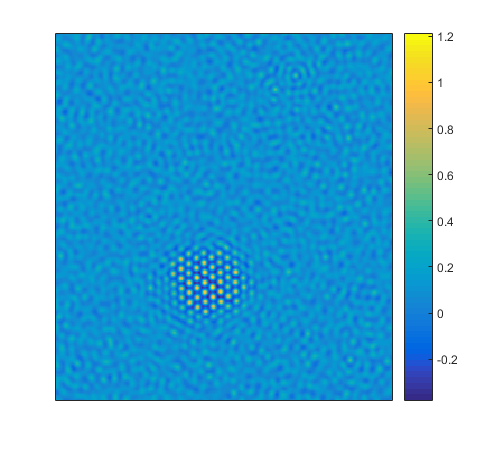
\includegraphics[width=0.5\textwidth]{fig_pfc/pfc_nuc1}
}
\subfloat[]
{
    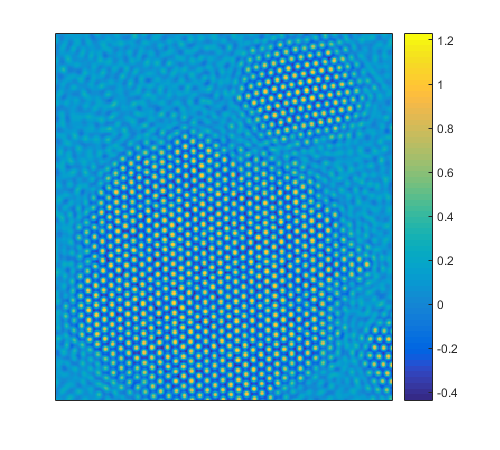
\includegraphics[width=0.5\textwidth]{fig_pfc/pfc_nuc2}
}
    \caption{Nucleation in a PFC simulation. Images ordered by simulation time elapsed. Parameters chosen were $B^x=1.00$, $B^l=1.10$, $n_o=0.1$, and $N_a=0.2$. (a) a solid nucleus appears in the middle of liquid phase (at simulation time $t=750$), (b) the first nucleus grows while other nuclei continue appearing (at $t=1250$).}\label{fig:pfc_example_nucleation}
\end{figure}

Conversely, for a large drop of $\Delta B$, the energy barrier between liquid and solid phases disappears. This leads to the system undergoing phase transition spontaneously and at all points in space simultaneously, as it decomposes spinodally into a ratio of solid and liquid volume predicted by the phase diagram at that point of parameter space. Figure \ref{fig:pfc_example_spinodal} shows a PFC simulation undergoing spinodal decomposition, without the need for thermal fluctuations.

\begin{figure}[h]
    \centering
\subfloat[]
{
    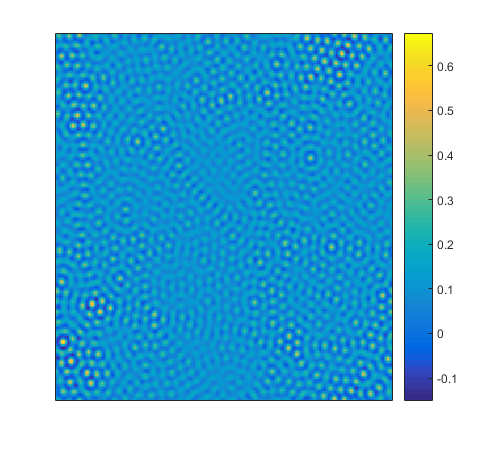
\includegraphics[width=0.5\textwidth]{fig_pfc/pfc_spi1}
}
\subfloat[]
{
    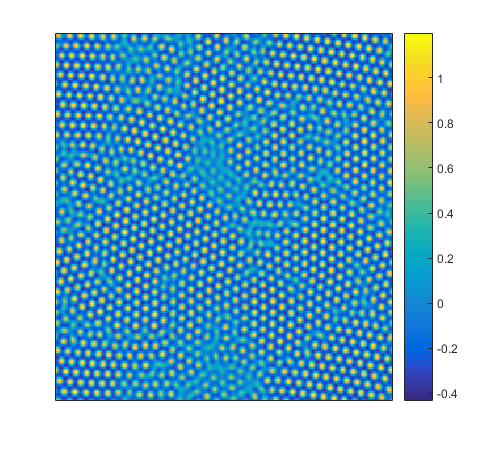
\includegraphics[width=0.5\textwidth]{fig_pfc/pfc_spi3}
}
    \caption{Spinodal decomposition in a PFC simulation. Images ordered by simulation time elapsed. Parameters chosen were $B^x=1.00$, $B^l=1.08$, $n_o=0.1$, and $N_a=0$. Numerical noise on the order of $10^{-7}$ was included in the initial state of the system, to break the initial symmetry. }\label{fig:pfc_example_spinodal}
\end{figure}

The precise $\Delta B$ at which behavior changes from nucleation-based phase transition to spinodal decomposition can be determined by calculating the linear stability of the phase field with respect to fluctuations. We do so by considering a perturbation from the liquid state,
%%
\begin{equation}\label{eq:perturb_n}
n(\vec{x},t) = n_o + \delta n(\vec{x},t)
\end{equation}
%%
where $\delta n(\vec{x},t)$ is the perturbation. Substituting this into equation \ref{eq:pfc_dynamics_dimensionless_final}, neglecting the noise term, and isolating the terms of order $\delta n$ gives
%%
\begin{equation}
\begin{split}
\frac{\partial \delta n}{\partial t} &= \Gamma \nabla^2 \left(B^x (2\nabla^2+\nabla^4)\delta n +g'(n_o)\delta n \right)\\ &= \Gamma \nabla^2 \left(B^x (2\nabla^2+\nabla^4) + B^l-2tn_o+3vn_o^2 \right)\delta n
\end{split}
\end{equation}
%%
where we have defined $g(n)=B^l n -tn^2 +vn^3$ and then Taylor expanded $g(n_o+\delta n)$ to order $\delta n$. Transforming the above to Fourier space gives
%%
\begin{equation}\label{eq:perturb_n_dynamics_fourier}
\frac{\partial \delta \hat{n}_k}{\partial t} =  -\Gamma k^2 \left(B^x (-2k^2+k^4) + B^l-2tn_o+3vn_o^2 \right)\delta \hat{n}_k
\end{equation}
%%

Equation \ref{eq:perturb_n_dynamics_fourier} is a first order ordinary differential equation with solution
%%
\begin{equation}\label{eq:perturn_ode_sol}
\begin{split}
\delta\hat{n}_k(t) &= \exp\left\{-\Gamma k^2 \left(B^x (-2k^2+k^4) + B^l-2tn_o+3vn_o^2 \right)t\right\} \delta\hat{n}_k(t=0)\\&\equiv e^{\gamma_k t}\, \delta\hat{n}_k(t=0)
\end{split}
\end{equation}
%%
for the defined coefficient $\gamma_k$. We see that, when no other fluctuations are present, the $k$th Fourier mode of the perturbation $\delta n$ will grow if and only if $\gamma_k > 0$. Taking the parameter $\Gamma$ to be positive (as it is a dimensionless solute mobility parameter), we find that having $\gamma_k > 0$ for some non-empty subset of available $k$ modes requires
%%
\begin{equation}\label{eq:pfc_spinodal_requirement}
\Delta B < 2tn_o -3vn_o^2
\end{equation}
%%

Although not all $k$ modes will be unstable to perturbation for a given set of parameters satisfying equation \ref{eq:pfc_spinodal_requirement}, having a non-empty subset of these modes be unstable is sufficient for the system to be unstable as a whole, since the nonlinear nature of the PFC model's time-evolution PDE ensures that any fluctuation will eventually spread to all $k$ modes due to nonlinear mode coupling. Equation \ref{eq:pfc_spinodal_requirement} thus gives the region of the PFC's phase diagram where an arbitrarily small fluctuation from the liquid state will always grow, resulting in phase transition. This is a characteristic of spinodal decomposition, where there exists no energy barrier between the liquid and solid phases. The remaining region of the phase diagram requires nucleation for any phase transition to take place. We refer to the boundary between the nucleating and non-nucleating regions as the instability curve.

For the remainder of this thesis, we will focus only on nucleation. Any simulated PFC system will have parameters chosen such that the system is above its instability curve.








\chapter{\sf Classical Nucleation Theory}\label{ch:nucleation}


Consider a pure liquid material capable of undergoing phase transition to a crystalline solid state. The atoms of the disordered liquid phase undergo constant thermal fluctuations, occasionally stochastically arranging into a structure resembling a small grain of the crystalline solid. These grains can then proceed to either dissolve back into disordered liquid due to further fluctuations, or continue growing as more atoms attach to the original structure. If the liquid is above its melting temperature, the grains will always eventually dissociate into component liquid atoms. However, below the melting temperature, whether the grains are stable to fluctuations and continue growing or not depends on their size, density, shape, as well as other factors. Classical nucleation theory (CNT) \cite{hoyt_phasetransf,sear07} attempts to predict the rate of appearance of stable solid grains under the simplest possible assumptions for factors determining their stability.

We begin this chapter by presenting the basic assumptions and predictions of CNT, formulated for a two-dimensional system. We then take a short detour to introduce the general Fokker-Planck (FP) equation, which is followed by a description of the specific form of this equation used in CNT. The FP equation then provides an approximate form for the time-dependent nucleation rate predicted by CNT. We conclude with our expectations in applying CNT to nucleation in the PFC model, including problems we will face.




%%%%%%%%%%%%%%%%%%%%%%%%%%%%%%%%%%%%%%%%%%%%%%%%%%%%%%%%%%%%%%%%%%%%%%%%%%%%%%%%%%%%
\section{Work of formation}\label{sec:nuc_work}

In CNT, the interior of a solid grain is treated as consisting of bulk solid, with a sharp interface separating it from the liquid phase around. The `work of formation' $W$ is the free energy required to form such a grain from the original liquid phase. $W$ consists of a bulk term, which represents the difference between the free energies of the solid and liquid phase, as well as a surface term representing the energy penalty for the existence of an interface. We write
%%
\begin{equation}\label{eq:nuc_work}
W = V\Delta G + A\gamma
\end{equation}
%%
where $\Delta G$ is the difference in local free energy density between the initial and final phases, $\gamma$ is the interfacial energy density, $V$ is the volume of the grain and $A$ is its interfacial surface area. $\gamma$ is always of positive sign, as physical systems attempt to minimize the surface area between different phases. If the temperature of the liquid phase is above its melting point, the liquid phase is more favorable than the solid phase, leading to a positive $\Delta G$ and thus a $W$ increasing with grain size. Any grains stochastically appearing would then always dissolve back to liquid as the system relaxes to minimum energy. On the other hand, for a temperature below the melting point, the solid phase is favored, leading to a negative $\Delta G$. As surface area generally scales slower than volume as a grain's size increases, $W$ then exhibits a global maximum. This global maximum defines the nucleation energy barrier: any stochastically-forming grain large enough to surpass the position of the maximum is energetically favored to keep growing, and vice versa for grains that do not surpass the maximum. Figure \ref{fig:nuc_work} sketches $W$ and its two component terms in equation \ref{eq:nuc_work}.

\begin{figure}[h]
    \centering
\subfloat[]
{
    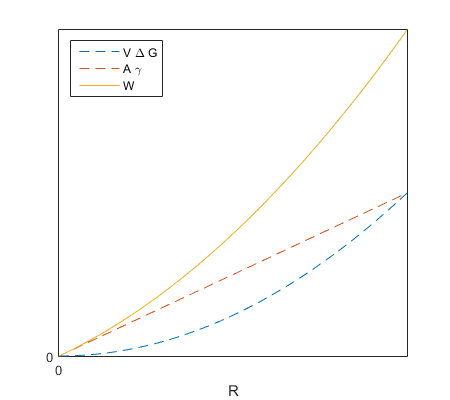
\includegraphics[width=0.5\textwidth]{fig_nuc/nuc_work1}
}
\subfloat[]
{
    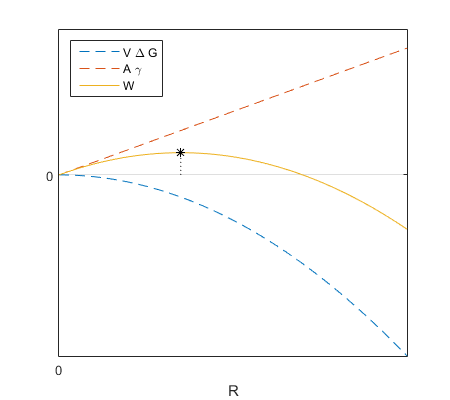
\includegraphics[width=0.5\textwidth]{fig_nuc/nuc_work2}
}
\caption{Sketch of $W$ and its component terms (y-axis) as a function of radius $R$ of the grain, assuming the grain is two-dimensional and circular. Blue is the bulk term, red is the interfacial term, and yellow is the sum $W$. (a) is for temperatures above the freezing point, (b) is for temperatures below the freezing point, also showing the height and position of the nucleation barrier in black.}\label{fig:nuc_work}
\end{figure}

Before continuing, we differentiate between two types of nucleation: homogeneous and heterogeneous. Heterogeneous nucleation occurs in contact with already-present surfaces, such as on the edges of the liquid's container, on earlier-formed solid grains, or on impurities suspended in the liquid. Homogeneous nucleation occurs in the middle of the liquid bulk, independently of position in the bulk (assuming a homogeneous liquid). The nucleation barrier for heterogeneous nucleation is always lower than for homogeneous, due to favorable attractive forces between the nucleating phase and the already-present surfaces \cite{sear07}. However, the number density of possible nucleation sites is much larger for homogeneous nucleation, as it can occur at any point in the liquid. The rate of heterogeneous nucleation is thus much more significant than homogeneous in most materials at small undercooling below the freezing point, where the homogeneous nucleation barrier is too large to realistically observe any homogeneous nucleation events, while homogeneous rate surpasses heterogeneous once sufficient undercooling is achieved. In this work we will concentrate on homogeneous nucleation, as its formulation is simpler and can be easily extended to the heterogeneous case by modifying the form of $W$.

As nature tends to minimize surface area, CNT assumes homogeneous nucleation results in spherical grains. The work of formation in a two-dimensional system can then be written as
%%
\begin{equation}\label{eq:nuc_work_circle}
W(R) = \pi R^2\Delta G + 2\pi R \gamma
\end{equation}
%%
where $R$ is the radius of the grain. The nucleation energy barrier is given by the maximum of equation \ref{eq:nuc_work_circle}, with value $W^*$ and position $R^*$ found to be
%%
\begin{equation}\label{eq:nuc_work_circle_max}
W^* = -\pi\frac{\gamma^2}{\Delta G}, \qquad R^* = -\frac{\gamma}{\Delta G}
\end{equation}
%%
recalling that $\Delta G <0$ below the freezing point. A critical nucleus is then defined to be a grain of radius $R^*$, and larger grains are termed post-critical nuclei.

CNT assumes that atoms in a grain have their mass evenly distributed throughout the grain. We can thus rewrite equation \ref{eq:nuc_work_circle} in terms of the number of atoms in the grain, giving
%%
\begin{equation}\label{eq:nuc_work_g}
W(g) = vg\Delta G + sg^{1/2} \gamma
\end{equation}
%%
where $g$ is the number of atoms, and $v$ and $s$ are the area and interfacial length of a two-dimensional grain consisting of 1 atom ($g=1$) respectively. The critical nucleus' number of atoms $g^*$ is then found similarly as in equation \ref{eq:nuc_work_circle_max}, giving
%%
\begin{equation}\label{eq:nuc_crit_num_g}
g^* = \left(-\frac{s\gamma}{2v\Delta G}\right)^2
\end{equation}
%%

%%%%%%%%%%%%%%%%%%%%%%%%%%%%%%%%%%%%%%%%%%%%%%%%%%%%%%%%%%%%%%%%%%%%%%%%%%%%%%%%%%%%
\section{Steady state rate of nucleation}\label{sec:nuc_steadyrate}

In CNT, each atom in the liquid can aggregate more atoms around it to form a grain, and hence each atom is a possible homogeneous nucleation site. Let $\rho_1$ be the number density of individual atoms in the liquid, equivalently the number density of grains of size $g=1$. If the liquid is allowed to remain at a specific temperature long enough to reach a `steady state', the number density of grains formed due to fluctuations and consisting of $g$ atoms can be written as
%%
\begin{equation}\label{eq:nuc_grainsdist_ss}
\rho(g) = \rho_1 \exp\left(-\frac{W(g)}{k_B T}\right)
\end{equation}
%%
where grains requiring a work of formation of $W(g)$ are assumed to follow the appropriate Boltzmann distribution. Equation \ref{eq:nuc_grainsdist_ss} neglects grains that stabilize and keep growing due to being post-critical after stochastically forming.

CNT predicts the `steady state' rate of homogeneous nucleation per unit volume to be \cite{hoyt_phasetransf}
%%
\begin{equation}\label{eq:nuc_rate_ss}
J_{ss} = Zj^*\rho(g^*)= Zj^* \rho_1\exp\left(-\frac{W^*}{k_B T}\right)
\end{equation}
%%
where $j^*$ is the rate of attachment of atoms to a critical nucleus, and $Z$ is the so-called Zeldovich factor. Multiplying the number density $\rho(g^*)$ of exactly critical nuclei by $j^*$ gives the rate that these critical nuclei become post-critical. The Zeldovich factor is a value less than 1 that accounts for the possibility of fluctuations causing a post-critical nucleus to lose enough atoms to revert to pre-critical, which is known to scale in two dimensional systems as
%%
\begin{equation}\label{eq:nuc_Z_scaling}
Z \propto \left(-\frac{1}{k_B T}\frac{\partial^2 W}{\partial g^2}\Bigr|_{g=g^*}\right)^{1/2} \propto \left(\frac{(g^*)^{-3/2}\gamma}{k_B T}\right)^{1/2} \propto \frac{(-\Delta G)^{3/2}}{\gamma  (k_B T)^{1/2}}
\end{equation}
%%

In general, the exponential factor in equation \ref{eq:nuc_rate_ss} is the most significant in determining the rate of nucleation, though the attachment rate $j^*$ might also be of significant effect depending on the material \cite{hoyt_phasetransf}.

As an aside, the rate of heterogeneous nucleation can be obtained by switching $\rho$ to the number density of heterogeneous nucleation sites (such as impurity particles) and $W^*$ to the appropriate work of formation for a heterogeneous nucleus.

We note that the term `steady state' is misleading, in that it implies the system is at some sort of equilibrium when in fact a liquid capable of phase transition through nucleation is a metastable phase. Rather, `steady state' is to be understood as an assumption that the liquid has been at its current temperature for long enough that nucleation happens at a constant rate. In general, a liquid that starts at a temperature above its freezing point and is then rapidly quenched to below the freezing point will not instantly exhibit this nucleation rate. Instead, a certain amount of time, known as the `incubation' time, must pass before the nucleation rate begins approaching its steady state value. To obtain the time-dependent rate of nucleation, we must define a time-dependent version of the grain number density given in equation \ref{eq:nuc_grainsdist_ss}, as well as a corresponding time-evolution PDE for that density. This PDE is a specific form of the Fokker-Planck (FP) equation, introduced in the following sections.

%%%%%%%%%%%%%%%%%%%%%%%%%%%%%%%%%%%%%%%%%%%%%%%%%%%%%%%%%%%%%%%%%%%%%%%%%%%%%%%%%%%%
\section{The FP equation in general}\label{sec:nuc_fopl_general}

Consider a set of stochastic real scalar variables each corresponding to a point in time, $\{X(t) : t \in \mathbb{R} \}$. This set can represent a stochastic physical process, such as the position of a particle moving in a random direction at any given time. Let $P(X,t)$ be the probability density of $X(t)$, meaning the probability that $a\leq X(t) \leq b$ for some $t$ is
%%
\begin{equation}
\mathrm{Pr}[a\leq X(t) \leq b,t]=\int_a^b P(X,t)dX
\end{equation}
%%

We assume the stochastic process represented by $X(t)$ is a `Markov process': Given the probability density $P(X,t_1)$ at time $t_1$, all future probability densities $P(X,t_2)$ for $t_2>t_1$ can be determined with no knowledge of past probability densities $P(X,t_0)$ for $t_0<t_1$. Heuristically, this can be seen as requiring the process to be deterministic in a specific sense: Despite the variables $X(t)$ not being deterministic themselves, the probability density $P(X,t)$ evolves deterministically through time.

The goal is to obtain the time-evolution PDE for the probability density function $P(X,t)$, though the general derivation \cite{kolpas07,gardiner_stochastic} of this PDE is outside the scope of this work. The full derivation allows a PDE of arbitrary order in $X$, but here we truncate the PDE to 2nd order in $X$, giving
%%
\begin{equation}\label{eq:fopl_general}
\frac{\partial P(X,t)}{\partial t}= \frac{\partial^2}{\partial X^2} (D(X,t)P(X,t)) -  \frac{\partial}{\partial X}(\mu(X,t)P(X,t))
\end{equation}
%%
where the coefficients $D(X,t)$ and $\mu(X,t)$ correspond in many physical systems to the diffusion coefficient and the drift coefficient respectively. This PDE is the general Fokker-Planck equation for a one-dimensional stochastic variable.

The prototypical example utilizing equation \ref{eq:fopl_general} would be Brownian motion of a particle, such as the motion exhibited by a pollen particle suspended in water. Such a particle moves in a random direction at any given point in time as water molecules bump into it. This motion can be modeled as a random walk: Let $X(t)$ be the one-dimensional position at time $t$ of a particle that moves every time interval $\tau$ a distance of $\lambda \pm \epsilon$ with equal probability for either sign. It can be shown \cite{gardiner_stochastic} that, in the limit where $\tau$ is small compared to the total time considered, the probability density $P(X,t)$ of the particle's position evolves according to equation \ref{eq:fopl_general} with constant coefficients $D=\epsilon^2/2\tau$ and $\mu=\lambda/\tau$. Figure \ref{fig:randwalk1} shows the paths taken by a few such particles starting from the same initial position. Figure \ref{fig:randwalk2} shows the corresponding position probability density evolving through time, with the initial position represented by a Dirac $\delta$ function at the starting time. As mentioned above, the FP equation thus allows us to calculate the particle's position probability distribution deterministically, despite the particle's motion being non-deterministic. In the next section, we will similarly determine the probabilistic evolution of a grain of solid in a fluctuating liquid, as atoms randomly attach to and detach from the grain.

\begin{figure}[h]
    \centering
\subfloat[]
{
    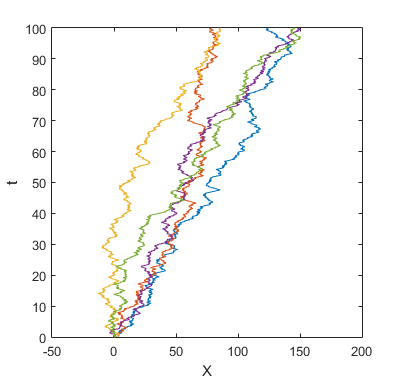
\includegraphics[width=0.5\textwidth]{fig_nuc/randwalk1}
    \label{fig:randwalk1}
}
\subfloat[]
{
    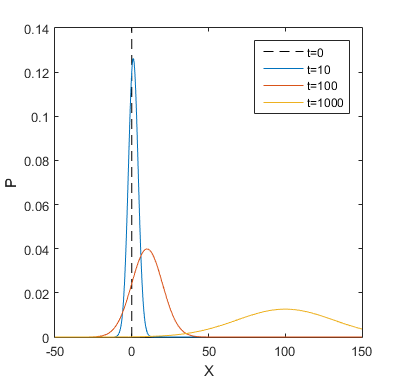
\includegraphics[width=0.5\textwidth]{fig_nuc/randwalk2}
    \label{fig:randwalk2}
}
\caption{(a) The positions $X(t)$ for 5 particles undergoing random walks with $\tau=0.1$, $\lambda=0.1$, $\epsilon=1$, and initial position $X(0)=0$. (b) The probability density for the position of these same particles, at different times.}
\end{figure}

It should be noted that the FP equation for Brownian motion gives the probability distribution for the position of a \textit{single} particle. If we are instead interested in the positions of a large amount of particles present in the same system, we must make the assumption that the particles do not interact with each other as they move. With that assumption, the FP equation can be used for the exact time-evolution of the number density of the Brownian particles. A similar non-interaction requirement proves to be problematic for the application of CNT to the PFC model, as will be discussed in section \ref{sec:nuc_cnt_pfc}.



%%%%%%%%%%%%%%%%%%%%%%%%%%%%%%%%%%%%%%%%%%%%%%%%%%%%%%%%%%%%%%%%%%%%%%%%%%%%%%%%%%%%
\section{The FP equation in CNT}\label{sec:nuc_fopl_nucleation}

Define the time-dependent grain number density in a nucleating liquid phase to be $c(g,t)$, assumed to satisfy $c(g,\infty)=\rho(g)$. Assuming non-interaction between the grains in the liquid, a specific form of the FP equation will give the time-evolution of $c(g,t)$ in the one-dimensional size-space $g$. This FP equation can be derived directly from simple CNT assumptions without the general derivation mentioned in the previous section \cite{hoyt_phasetransf,yoo87,shi90}.

The fluctuations that form grains will now be represented by rates of attachment and detachment of atoms to and from grains. Let $j(g)$ be the rate at which grains of size $g$ grow to $g+1$ by gaining 1 more atom, and conversely $l(g)$ the rate of shrinking from $g$ to $g-1$. The total `flux' of grains in size-space is written as%The specific form of these rates depends on the material under consideration, but in general scales proportionally to the interface length (or area in 3D) of a grain of size $g$. 
%%
\begin{equation}\label{eq:nuc_flux_total}
J(g,t)=j(g)c(g,t)-l(g+1)c(g+1,t)
\end{equation}
%%

At $t=\infty$, the flux must be zero to achieve nucleation steady state. Setting $J(g,\infty)=0$ in equation \ref{eq:nuc_flux_total} gives
%%
\begin{equation}
l(g+1)= \frac{j(g)c(g,\infty)}{c(g+1,\infty)}=\frac{j(g)\rho(g)}{\rho(g+1)}
\end{equation}
%%
which allows rewriting equation \ref{eq:nuc_flux_total} as
%%
\begin{equation}\label{eq:nuc_flux_reduced}
\begin{split}
J(g,t)&=j(g)\left[c(g,t)-\frac{\rho(g)}{\rho(g+1)}c(g+1,t)\right]\\&=j(g)\rho(g)\left[\frac{c(g,t)}{\rho(g)}-\frac{c(g+1,t)}{\rho(g+1)}\right]\\&=-j(g)\rho(g)\frac{\partial}{\partial g}\left[\frac{c(g,t)}{\rho(g)}\right]
\end{split}
\end{equation}
%%
where in the last step the difference was approximated by the appropriate partial derivative.

The growth rate $j(g)$ for a two-dimensional liquid undergoing transition to a crystalline solid is expected to scale as \cite{turnbull49}
%%
\begin{equation}\label{eq:nuc_attachmentrate}
j(g) \propto g^{1/2} k_B T \exp\left(-\frac{\Delta G_A}{k_B T}\right)
\end{equation}
%%
where $\Delta G_A$ is the activation energy needed for an atom to cross the liquid-solid interface to attach to the grain. %For physical systems such as water below its freezing point \cite{jeffery97}, $\Delta G_A$ is estimated to decrease with increasing temperature.

Grains are assumed to all originate as grains of size $g=1$ (i.e. individual atoms). This gives the initial condition of the system to be $c(g,t=0)=\rho_1\delta(g-1)$, recalling that $\rho_1$ is the number of homogeneous nucleation sites available as well as the number density of individual atoms. Grains do not appear or disappear after initial conditions of the system are set, only being allowed to grow and shrink. Conservation of number density in size-space then requires a continuity equation, given as
%%
\begin{equation}\label{eq:nuc_continuity}
\frac{\partial c}{\partial t}=-\frac{\partial J}{\partial g}
\end{equation}
%%

Plugging equation \ref{eq:nuc_continuity} into \ref{eq:nuc_flux_reduced} yields CNT's FP equation, written as
%%
\begin{equation}\label{eq:nuc_fopl}
\frac{\partial c(g,t)}{\partial t}=\frac{\partial}{\partial g}\left[j(g)\rho(g)\frac{\partial}{\partial g}\left(\frac{c(g,t)}{\rho(g)}\right)\right]
\end{equation}
%%

%%%%%%%%%%%%%%%%%%%%%%%%%%%%%%%%%%%%%%%%%%%%%%%%%%%%%%%%%%%%%%%%%%%%%%%%%%%%%%%%%%%%
\section{Analytical approximations for the nucleation rate and incubation time}\label{sec:nuc_fopl_sol}

The time-dependent nucleation rate in the nucleating liquid phase is defined to be the flux in size-space of grains at the critical nucleus size $g^*$, which is $J(g^*,t)$ given by equation \ref{eq:nuc_flux_reduced}. An approximate form for this rate, with the above mentioned initial condition, is obtained by Shi, Seinfeld and Okuyama \cite{shi90} by solving the FP equation \ref{eq:nuc_fopl} using singular perturbation methods. This rate is
%%
\begin{equation}\label{eq:nuc_crit_flux}
J^*(t)=J(g^*,t)=J_{ss} \exp\left[-\exp\left(-2\frac{t}{\tau}+2\lambda\right)\right]
\end{equation}
%%
where we have renamed the rate to $J^*(t)$ for convenience. $J_{ss}$ is the steady state nucleation rate given in equation \ref{eq:nuc_rate_ss}, and $\tau$ and $\lambda$ are values that depend on $g^*$ and determine the incubation time before steady state is achieved. In two dimensions, these are calculated to scale as
%%
\begin{equation}\label{eq:nuc_tau_scaling}
\tau \propto \frac{1}{Z^2 j(g^*)}
\end{equation}
%%
%%
\begin{equation}\label{eq:nuc_lambda_scaling}
\lambda \propto  (g^*)^{-1/2} -1 + \ln\left(Zg^*(1-(g^*)^{-1/2})\right) +\ln\left(2\sqrt{\pi}\right)%O(\ln(g^*))
\end{equation}
%%

It proves to be numerically (and experimentally) easier to calculate the number of post-critical nuclei in a simulated system than it is to directly calculate their rate of appearance. Hence, we derive the time-dependent number density of post-critical nuclei by taking the integral of equation \ref{eq:nuc_crit_flux}. This gives
%%
\begin{equation}\label{eq:nuc_crit_numdens}
I^*(t)=\int_0^t J^*(s)ds=- \frac{J_{ss} \tau}{2} \mathrm{Ei}\left[-\exp\left(-2\frac{t}{\tau}+2\lambda\right)\right]
\end{equation}
%%
where it is implicit that $I^*(t)$ still depends on the critical nucleus size $g^*$, and $\mathrm{Ei}(.)$ is the exponential integral function, defined as
%%
\begin{equation}
\mathrm{Ei}(x)=\int_{-\infty}^x\frac{e^s}{s}ds
\end{equation}
%%

It is not immediately clear from the forms of equations \ref{eq:nuc_crit_flux} and \ref{eq:nuc_crit_numdens} what value should be considered the incubation time, as both $\tau$ and $\lambda$ affect the time needed to reach steady state nucleation rate $J_{ss}$. In this work, we will define the incubation time geometrically, in a manner similar to experimental works such as \cite{legoues84}. As $t \rightarrow \infty$, we calculate that $I^*(t)$ asymptotes to a line given by
%%
\begin{equation}\label{eq:nuc_crit_numdens_asymptote}
I^*(t) \approx J_{ss} ( t - \tau(\lambda+\gamma_{e}/2) )
\end{equation}
%%
where $\gamma_{e}$ is the Euler-Mascheroni constant. The intercept of this line with the horizontal axis is then taken to be the incubation time, written as
%%
\begin{equation}\label{eq:nuc_incubationtime}
t^*=\tau(\lambda+\gamma_{e}/2)
\end{equation}
%%

Figure \ref{fig:nuc_rates_fixedinc} sketches $J^*(t)$ and $I^*(t)$ for a fixed incubation time $t^*$ as $\tau$ and $\lambda$ are varied. We observe that taking $\tau \rightarrow 0$ with $t^*$ fixed leads to $J^*(t)$ approaching a step function of form
%%
\begin{equation}
J^*(t)\approx
\begin{cases}
    J_{ss}& \text{if } t\geq t^*\\
    0              & \text{otherwise}
\end{cases}
\end{equation}
%%

\begin{figure}[h]
    \centering
\subfloat[]
{
    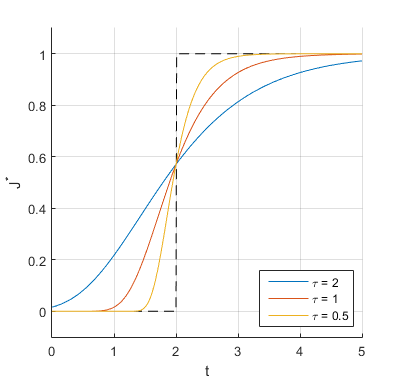
\includegraphics[width=0.5\textwidth]{fig_nuc/nucrates_fixedtinc_J}
}
\subfloat[]
{
    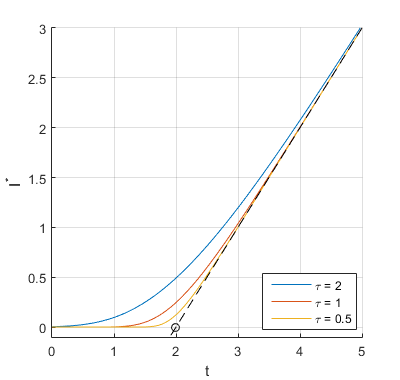
\includegraphics[width=0.5\textwidth]{fig_nuc/nucrates_fixedtinc_I}\label{fig:nuc_rates_fixedinc_b}
}
\caption{(a) Sketch of $J^*(t)$ for $J_{ss}=1$ and $t^*=2$ fixed while $\tau$ varies. Black shows the step function for $\tau \rightarrow 0$. (b) Sketch of $I^*(t)$ for $J_{ss}=1$ and $t^*=2$ fixed while $\tau$ varies. Black shows the asymptote line, and its intersection with the horizontal axis is shown by the black circle.}\label{fig:nuc_rates_fixedinc}
\end{figure}

Finally, we estimate the predicted scalings of $J_{ss}$ and $t^*$ by combining equations \ref{eq:nuc_work_circle_max}, \ref{eq:nuc_crit_num_g}, \ref{eq:nuc_rate_ss}, \ref{eq:nuc_Z_scaling}, \ref{eq:nuc_attachmentrate}, \ref{eq:nuc_tau_scaling}, \ref{eq:nuc_lambda_scaling}, and \ref{eq:nuc_incubationtime}. We find
%%
\begin{equation}\label{eq:nuc_Jss_scaling}
J_{ss} \propto (-\Delta G \, k_B T)^{1/2}\exp\left(-\frac{\Delta G_A}{k_B T}\right)\exp\left(-\frac{\pi}{k_B T}\frac{\gamma^2}{(-\Delta G)}\right)
\end{equation}
%%
%%
\begin{equation}\label{eq:nuc_tinc_scaling}
t^* \propto \left[\frac{1}{(-\Delta G)}+K\frac{\gamma}{(\Delta G)^2}\right]\exp\left(+\frac{\Delta G_A}{k_B T}\right)
\end{equation}
%%
where we have expressed the scalings in terms of the local free energy density difference $\Delta G$ between the solid and liquid phase, the interfacial energy density $\gamma$ of a grain, the temperature factor $k_B T$, and the atomic-attachment activation energy $\Delta G_A$. We also defined
%%
\begin{equation}
K \propto \gamma_e/2-1+ \ln\left(2\sqrt{\pi}\right)+\ln\left(\frac{\gamma}{(-\Delta G \, k_B T)^{1/2}}  \left(1-\frac{(-\Delta G)}{k_B T}\right)  \right) 
%K = \lambda - (g^*)^{-1/2}
\end{equation}
%%
which we will take to be approximately constant due to the slow variation of the logarithmic function. The sign of $K$ depends on the sign of $\lambda$, which in turn can be seen from figure \ref{fig:nuc_rates_fixedinc} and equation \ref{eq:nuc_incubationtime} to depend on how quickly the time-dependent nucleation rate increases from zero to $J_{ss}$.


%%%%%%%%%%%%%%%%%%%%%%%%%%%%%%%%%%%%%%%%%%%%%%%%%%%%%%%%%%%%%%%%%%%%%%%%%%%%%%%%%%%%
\section{Expectations in comparing CNT to nucleation in the PFC model}\label{sec:nuc_cnt_pfc}

To compare nucleation in the PFC model to the predictions of CNT, we will obtain the number density of post-critical nuclei $I^*(t)$ in different simulated PFC systems. This number density will be used to calculate $J_{ss}$ and $t^*$ geometrically as described in the previous section. We will then examine the scaling of these two values in the PFC model and compare them to equations \ref{eq:nuc_Jss_scaling} and \ref{eq:nuc_tinc_scaling}. Chapter \ref{ch:numerics} will detail the numerics used to accomplish these goals, while chapter \ref{ch:results} will showcase the corresponding results. In this section, we preemptively describe the difficulties we expect to encounter due to the assumptions made by CNT in its derivations.

The first difficulty will relate to the finite size of the simulated systems. As CNT assumes grains do not interact and also assumes the number density of single atoms (equivalently, homogeneous nucleation sites) $\rho_1$ is constant through time, its predictions are expected to only hold in early times for the PFC model simulations, before a significant fraction of the liquid phase has transitioned to the solid phase. For this reason, we will be unable to ascertain that the $I^*(t)$ obtained from the simulations has reached its predicted late-time asymptotic value before tapering off due to finite size limits. As such, calculating $J_{ss}$ and $t^*$ geometrically from the presumed asymptote line are only guaranteed to provide lower bounds for these values, rather than exact results.

A second and more subtle difficulty is found in CNT's use of a single variable to describe grains, the number of atoms $g$ in a grain. In both the PFC model and other nucleating systems, this can prove to be an oversimplification, as shape, density, and interface width of the grains can vary independently during the formation process. See for example \cite{lutsko15} where nucleation in globular protein systems is assumed to depend both on interior density and radius of the grains. It is then unclear whether the definitions of $\gamma$ and $\Delta G$ are sound for small pre-critical grains, as $\gamma$ assumes a sharp interface and $\Delta G$ assumes inner grain density equal to the final solid bulk density. In addition, due to vibrational-timescale fluctuations being averaged out in the PFC model, it is unclear whether the assumption of single-atom attachment rate as from equation \ref{eq:nuc_attachmentrate} is a reasonable approximation, and no direct equivalent to the activation energy $\Delta G_A$ is available in this model. Furthermore, as the PFC model's systems consist of a continuous density field rather than discrete atoms, it is feasible that the formation of grains involves fluctuations in the field that do not follow the expected lattice structure at early times, before the grains stabilize. See for example \cite{toth11} where the authors observe what appears to be amorphous structure appearing in the PFC model preceding a crystalline phase, though they are unable to conclude whether this structure represents a separate amorphous phase or very small and tightly packed crystal grains. As part of the discussion of our results, we will attempt to numerically calculate an approximation for the form of the critical nucleus in the PFC model. We will also examine the behavior of the density field during the early formation stage of the grains. These undertakings will be used as guides to whether CNT assumptions are reasonable. We will continue assuming the definitions of $\gamma$ and $\Delta G$ hold, at least in some approximate manner, when examining the scalings of $J_{ss}$ and $t^*$.

The final hurdle relates to the two different temperature parameters that are defined in the PFC model: the effective temperature $\Delta B$ obtained from the parameters in the model's free energy functional in equation \ref{eq:PFC_energyFunctional}, and the fluctuation temperature $T_r$ that follows from the fluctuation-dissipation theorem inherent in defining fluctuations in equation \ref{eq:pfc_noise_dimensionless}. While the authors of \cite{kocher16} effectively couple the values of these two temperature parameters as the other model parameters are varied, there is no definitive way to decide which temperature dependencies of values in the CNT scaling predictions of equations \ref{eq:nuc_Jss_scaling} and \ref{eq:nuc_tinc_scaling} correspond to each of $\Delta B$ and $T_r$. We make the following assumptions related to temperature dependence: Factors of $k_B T$ appearing in the exponential terms $\exp(-\Delta G_A/k_B T)$ and $\exp(-W^*/k_B T)$ are taken to be equivalent to $T_r$, as these exponential terms are based on Boltzmann distribution arguments. We also assume that the temperature dependence of $\Delta G$ is related only to $\Delta B$ and can be approximated from the difference of the local free energy densities of solid and liquid bulks obtained in section \ref{sec:pfc_phasediag}. Further, interfacial energies of stable interfaces in the PFC model are known \cite{provatas_coms} to decrease slowly as $\Delta B$ increases, and we take $\gamma$ to vary as such. Finally, for physical systems such as water below its freezing point \cite{jeffery97}, $\Delta G_A$ is estimated to decrease with increasing temperature. We thus assume that, if its effects are present in the PFC model, $\Delta G_A$ decreases with one or both of the temperature parameters, though its exact dependence is unknown. We will attempt to evaluate these assumptions based on the results we obtain.

%%%%%%%%%%%%%%%%%%%%%%%%%%%%%%%%%%%%%%%%%%%%%%%%%%%%%%%%%%%%%%%%%%%%%%%%%%%%%%%%%%%%

















\chapter{\sf Numerical Methods}\label{ch:numerics}

This chapter begins with the derivation of the time-stepping equation used to simulate the PFC model's dynamics. Then, this equation's discretization and implementation are described. Following that, the procedure for calculating nucleation rates is presented. Finally, numerical tools for analyzing the early stages of grain formation, including the form of critical nuclei, are developed.

%%%%%%%%%%%%%%%%%%%%%%%%%%%%%%%%%%%%%%%%%%%%%%%%%%%%%%%%%%%%%%%%%%%%%%%%%%%%%%%%%%%%
\section{Semi-implicit Fourier space method for solving PFC dynamics}\label{sec:num_pfc}

We obtain the time-stepping equations for the PFC model's dynamics using a semi-implicit Fourier space method \cite{provatas_PFC}. Begin by rewriting equation \ref{eq:pfc_dynamics_dimensionless_final} as
%%
\begin{equation}\label{eq:num_rewritten_pfc}
\frac{\partial n}{\partial t} = Ln + \nabla^2 N(n) + R
\end{equation}
%%
where $L=\nabla^2(B^l +B^x (2\nabla^2+\nabla^4))$, $N=-tn^2+vn^3$, and $R=\nabla \cdot \vec\xi$. We have taken $\Gamma=1$ for all our simulations. We assume the nonlinear term $N(n)$ and the noise term $R$ are calculated in real space at each time step. We take the Fourier transform of \ref{eq:num_rewritten_pfc}, giving
%%
\begin{equation}\label{eq:num_rewritten_pfc_fourier}
\frac{\partial \hat{n}_k}{\partial t} = \hat{L}_k \hat{n}_k - k^2 \hat{N}_k + \hat{R}_k
\end{equation}
%%
where $\hat{L}_k = - k^2(B^l +B^x (-2k^2+k^4))$, $\hat{N}_k$ and $\hat{R}_k$ are the respective transforms of $N$ and $R$, and $k^2=(k_x^2+k_y^2)$ is the wavevector's squared magnitude.

Approximating equation \ref{eq:num_rewritten_pfc_fourier} to be a first-order ordinary differential equation in $\hat{n}_k$, and defining $\hat{D}_k(t)=- k^2 \hat{N}_k + \hat{R}_k$, we write its solution as
%%
\begin{equation}\label{eq:num_pfcfourier_odesol}
\hat{n}_k(t)=\hat{n}_k(0) + e^{\hat{L}_k t}\int_0^t e^{-\hat{L}_k s}\hat{D}_k(s) ds
\end{equation}
%%
which can be rearranged at shifted time $t+\Delta t$ to give
%%
\begin{equation}\label{eq:num_pfcfourier_odesol_timeshift}
\begin{split}
\hat{n}_k(t+\Delta t)&=\hat{n}_k(0) + e^{\hat{L}_k (t+\Delta t)}\int_0^{t+\Delta t} e^{-\hat{L}_k s}\hat{D}_k(s) ds
\\&=\hat{n}_k(0) + e^{\hat{L}_k (t+\Delta t)} \left(\int_0^{t}+\int_t^{t+\Delta t} \right) e^{-\hat{L}_k s}\hat{D}_k(s) ds
\\&=e^{\hat{L}_k \Delta t}\hat{n}_k(t) + e^{\hat{L}_k (t+\Delta t)} \int_t^{t+\Delta t} e^{-\hat{L}_k s}\hat{D}_k(s) ds
\end{split}
\end{equation}
%%
The final approximation is to assume that $\hat{D}_k(t)$ varies much more slowly with $t$ than $e^{-\hat{L}_k t}$, leading us to write
%%
\begin{equation}
\int_t^{t+\Delta t} e^{-\hat{L}_k s}\hat{D}_k(s) ds \approx \hat{D}_k(t)\int_t^{t+\Delta t} e^{-\hat{L}_k s} ds = \frac{-e^{-\hat{L}_k t}(e^{-\hat{L}_k \Delta t}-1)}{\hat{L}_k}  \hat{D}_k(t)
\end{equation}
%%
which is then plugged into equation \ref{eq:num_pfcfourier_odesol_timeshift} to give the time-stepping equation
%%
\begin{equation}\label{eq:num_pfc_final}
\hat{n}_k(t+\Delta t)\approx e^{\hat{L}_k \Delta t}\hat{n}_k(t) +\frac{e^{\hat{L}_k \Delta t}-1}{\hat{L}_k} ( - k^2 \hat{N}_k + \hat{R}_k )
\end{equation}
%%

The advantage of using this semi-implicit method over a simpler method such as Euler time-stepping is that the semi-implicit method is stable for larger time steps $\Delta t$, allowing more efficient computation for the simulations.

%%%%%%%%%%%%%%%%%%%%%%%%%%%%%%%%%%%%%%%%%%%%%%%%%%%%%%%%%%%%%%%%%%%%%%%%%%%%%%%%%%%%
\section{Implementation of the time-stepping equation}\label{sec:num_discret}

Equation \ref{eq:num_pfc_final} is numerically calculated on a grid with spacing $dx=a/8$, where $a$ is the dimensionless lattice constant, and with time spacing $dt=1$. The size of the grid is $L \times L$, with $L$ a power of 2 chosen depending on the specific simulation run's goal (see following sections). Periodic boundary conditions are used on this grid.

The procedure to advance the simulation by one time step is as follows:
\begin{enumerate}
\item Generate the noise term $R=\nabla \cdot \vec\xi$ in real space. To do this, first generate two discrete fields $X$ and $Y$, corresponding to the two component fields of $\vec\xi$, whose points are uncorrelated random variables of Gaussian distribution, zero mean, and standard deviation $\sigma = N_a/\sqrt[]{dx^2dt}$. Then the discrete $R$ is given by
%%
\begin{equation}
R_{ij}=(X_{ij}-X_{i-1j}+Y_{ij}-Y_{ij-1})/dx
\end{equation}
%%
\item Calculate the nonlinear term $N=-tn^2+vn^3$ in real space.
\item Apply the well-known Fast Fourier Transform (FFT) algorithm on $N$ and $R$ to obtain $\hat{N}_k$ and $\hat{R}_k$.
\item Apply the noise spectrum cut-off discussed in section \ref{sec:pfc_dynamics}, by setting the grid points of the discrete $\hat{N}_k$ corresponding to wavenumbers with $k>2\pi/a$ to zero.
\item Calculate the new Fourier transformed discrete dimensionless density field $\hat{n}_k$ in Fourier space using equation \ref{eq:num_pfc_final}.
\item Apply the inverse FFT algorithm on $\hat{n}_k$ to obtain the real-space $n$, to be used in calculating the nonlinear term in the next time step.
\end{enumerate}

The code for this procedure is implemented in MATLAB, using that software's Parallel Computing Toolbox to enable computation on a Graphics Processing Unit (GPU). Early prototypes of the code where implemented in the C programming language, using the CUDA libraries to run the computationally-intensive subsets of the code on a GPU. Although the C version of the code showed speeds around $3\times$ that of the MATLAB code, the ease of implementation of analysis tools in MATLAB led to the eventual switch. The code ran on a laptop equipped with a NVIDIA GeForce GTX 960M GPU device.


%%%%%%%%%%%%%%%%%%%%%%%%%%%%%%%%%%%%%%%%%%%%%%%%%%%%%%%%%%%%%%%%%%%%%%%%%%%%%%%%%%%%
\section{Simulations for calculation of post-critical nuclei densities}\label{sec:num_rates}

For a given set of parameters $B^l$, $B^x$, $n_o$, and $N_a$, obtaining the PFC model's time-evolving post-critical nuclei densities involves averaging the results of a large number of simulation runs. Each simulation run has grid size given by $L=1024$, and as initial condition a system full of liquid, $n(\vec{x})=n_o$.

Every $N_{out}=50$ time steps (defined as one `output step') in a given run, the local maxima of the discretized field $n$ are obtained by comparing each grid point with its 8 neighbors. The maxima that surpass a chosen threshold are considered peaks of the periodic function $n$, and their positions are stored. The threshold is taken to be half the maximum deviation of the periodic function from the liquid average density, i.e. $n_o + 0.75\phi_s$ where $\phi_s$ was obtained in equation \ref{eq:freeEnergy_minima}. For what follows, these peaks are assumed to be the position of atoms in the crystal lattice of formed solid regions.

Each run is set to last until 90\% of the maximum possible number of peaks have formed. Assuming the chosen parameters place the system below the phase diagram's solidus, and knowing that the formed lattice structure is triangular with lattice constant $a$, we can calculate the maximum number $M_p$ of peaks that can appear in the simulation by dividing the total simulation area by the area of the lattice's unit cell, giving
%%
\begin{equation}
M_p = \frac{(dx\,L)^2}{(\sqrt[]{3}/2)a^2}
\end{equation}
%%

Once all runs are complete, the obtained peaks are used to count the number of nucleation events that occurred. To do so, the peaks must be grouped into separate clusters, representing individual crystal grains that have formed and possibly grown. The clusters must remain distinguishable even after their growth leads to impingement of their grain boundaries. 

\begin{figure}[!ht]
    \centering
\begin{tabular}{cccc}
\subfloat[]
{
    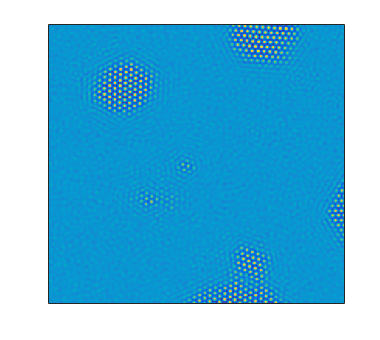
\includegraphics[width=0.5\textwidth]{fig_num/clustEx_1b}
}
&\subfloat[]
{
    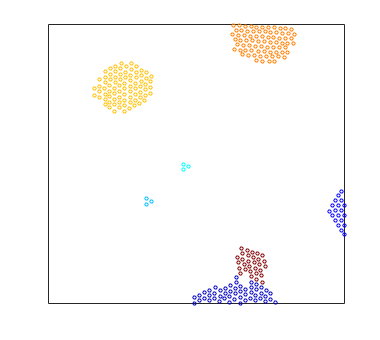
\includegraphics[width=0.5\textwidth]{fig_num/clustEx_1a}
}\\
\subfloat[]
{
    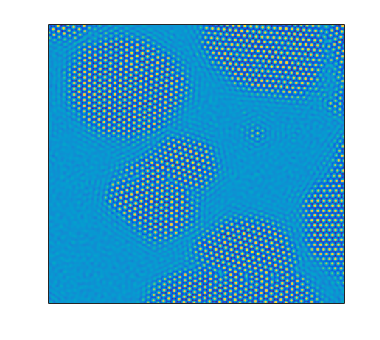
\includegraphics[width=0.5\textwidth]{fig_num/clustEx_2b}
}
&\subfloat[]
{
    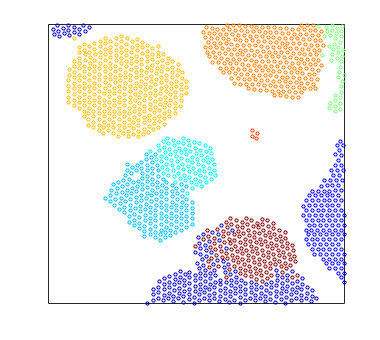
\includegraphics[width=0.5\textwidth]{fig_num/clustEx_2a}
}
\end{tabular}
    \caption{(a) and (c) show two snapshots of the density field $n$ in a small area of a simulation run, ordered by time. (b) and (d) show the corresponding detected peaks, grouped into clusters shown by color.}\label{fig:num_clustexample}
\end{figure}

Here we state our method for grouping peaks into clusters. Let $P(t)$ be the set of all peaks found at time $t$ in a specific run, and let $d(p_1,p_2)$ be the function which gives the distance between two peaks $p_1 , p_2 \in P(t)$. Let $C(t)$ be the set of all clusters at time $t$, with each of its elements consisting of a subset of $P(t)$ representing the peaks in a specific cluster. The procedure to determine $C(t)$ at a time $t$, given the set $P(t)$, is as follows: 
\begin{enumerate}
\item Set $C(t)=C(t-N_{out}dt)$, where $t-N_{out}dt$ is the time of the previous output step. If this is the first output step, set $C(t)$ to be the empty set.
\item For every $c \in C(t)$, remove peaks $p\in c$ where $p \notin P(t)$. This removes peaks that have vanished since the previous output step.
\item For every $p_1\in P(t)$ where $p_1$ belongs to no cluster in $C(t)$, check if $d(p_1,p_2)<3a$ for any peak $p_2\in c$ for any $c\in C(t)$. If so, add $p_1$ to cluster $c$. This adds peaks which appeared due to a previously-present growing cluster to that cluster. The distance value $3a$ was chosen to allow leeway for peaks appearing further than the lattice constant $a$ before merging fully with the cluster that generated them. This also accounts for some possible heterogeneous nucleation events, which we do not wish to count as separate clusters that would skew the homogeneous nucleation rate calculation. Repeat this step of the procedure until no $p_1$ is left that satisfies the distance requirement.
\item If there remains any $p\in P(t)$ that belong to no cluster of $C(t)$, choose one of these $p$ at random. Define a new cluster in $C(t)$ consisting of only that peak. Then return to step 3 of this procedure. This ensures that eventually all peaks are sorted into a cluster.
\end{enumerate}


Figure \ref{fig:num_clustexample} shows two zoomed-in snapshots of a simulation run, along with corresponding plots of the detected peaks grouped into clusters using the above method. Note that the method does not always perfectly separate impinging clusters at their lattice boundaries. This is not an issue as we are interested in the number of such distinguishable clusters, rather than their exact final size.

In our simulation runs, we observed that any cluster consisting of 3 or more detected peaks tended to keep growing far more often than shrinking. As such, we assume that clusters with 3 or more peaks represent post-critical nuclei. Note that this assumption does not imply that the exactly critical nuclei must have 3 atoms, as the detected peaks only account for peaks above the threshold defined previously, without accounting for other factors in the form of crystal grains that determines whether they are critical nuclei. The set of clusters $C(t)$ is then used to obtain the number of such nuclei in one run as a function of time. Summing this number over all runs that use the same set of parameters, and dividing by the total simulation area of all these runs, yields our value for the number of post-critical nuclei per area as a function of time. This value can then be compared to CNT's prediction for $I^*(t)$ as mentioned in section \ref{sec:nuc_cnt_pfc}.




%%%%%%%%%%%%%%%%%%%%%%%%%%%%%%%%%%%%%%%%%%%%%%%%%%%%%%%%%%%%%%%%%%%%%%%%%%%%%%%%%%%%
\section{Wave mode analysis}\label{sec:num_wave}

As described in section \ref{sec:pfc_1mode}, the PFC model's density field $n$ can be expanded in terms of three wave modes, corresponding to the lowest order reciprocal lattice vectors of the triangular lattice. In the solid phase, these three wave modes would have equal amplitude. However, it is unclear whether the amplitude of all three of these wave modes must fluctuate to a nonzero value simultaneously for a stable solid grain to form from a liquid phase, or whether the wave modes can separately appear and build up to a stable nucleus over time. To better understand this early stage of grain formation in terms of the wave modes, we here develop a method to quantify the relative amplitudes of the present modes at the positions and times where grains appear in the simulations. Our method expands on work by Singer and Singer \cite{singer06}, where a method is developed to visualize the orientation of crystal grains in a fully solidified system.

We construct a `test wavelet', whose density field is given by one of the solid phase's wave modes multiplied to a Gaussian envelope, written as
%%
\begin{equation}
n_{w}(\vec{x}) = Ne^{-|\vec{x}|^2/2\sigma^2}\cos(2\pi \vec{q}\cdot\vec{x})
\end{equation}
%%
where $\vec{q}$ is one of the lowest order reciprocal lattice vectors, $N$ is a normalization constant that ensures the integral over the area of the wavelet is unity, and the standard deviation of the Gaussian is chosen to be $\sigma=0.8a$ for $a$ the lattice constant. Figure \ref{fig:num_testWavelet} shows this test wavelet.

\begin{figure}[h]
\centering
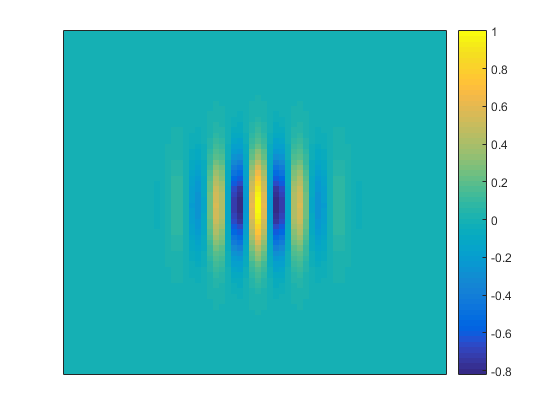
\includegraphics[width=0.5\textwidth]{fig_num/testWavelet.png}
\caption{The test wavelet for $\vec{q}$ chosen to be along the horizontal direction. The wavelet is shown unnormalized for clarity.}\label{fig:num_testWavelet}
\end{figure}

We convolve the test wavelet with the density field $n$ obtained from a simulation run, at a specific time $t$. This convolution enhances features of $n$ that exhibit the same structure as the wavelet. We then also apply a local averaging filter to smooth the field. The resulting filtered field's value provides at each spatial location a relative estimate of the amplitude of the wave mode corresponding to the wavelet's $\vec{q}$. By rotating the wavelet before applying this filtering process, the presence of a different wave mode can be examined. Figure \ref{fig:num_convtest} shows a snapshot of a simulation run, as well as the result of applying the filters on it for various rotations of the test wavelet. This filtering process can be applied every few time steps of a nucleation-rate simulation, for a range of rotation angles, to obtain the relative amplitude growth of wave modes at points where nucleation occurs.

\begin{figure}[!ht]
    \centering
\begin{tabular}{cccc}
\subfloat[]
{
    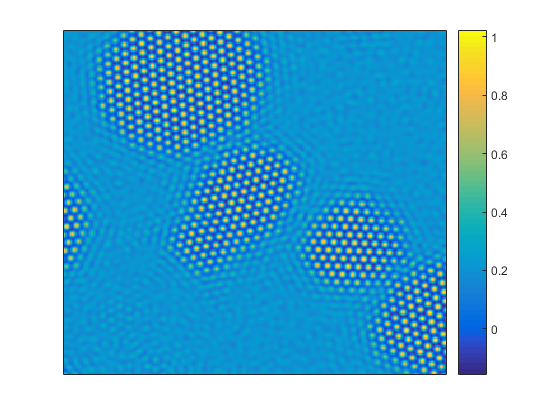
\includegraphics[width=0.5\textwidth]{fig_num/convtest1}
}
&\subfloat[]
{
    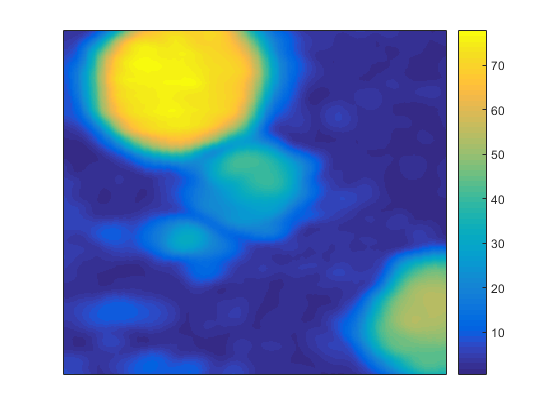
\includegraphics[width=0.5\textwidth]{fig_num/convtest2}
}\\
\subfloat[]
{
    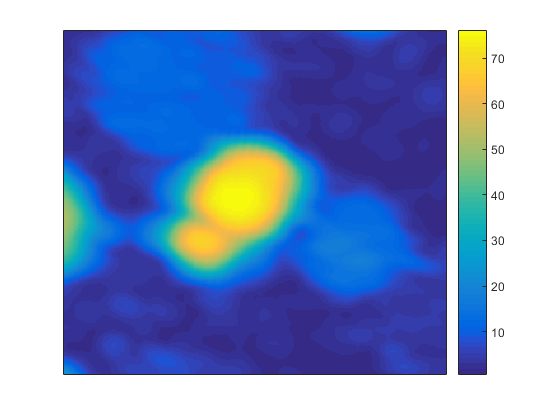
\includegraphics[width=0.5\textwidth]{fig_num/convtest3}
}
&\subfloat[]
{
    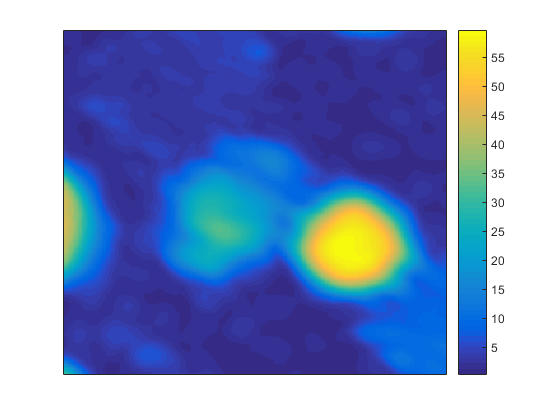
\includegraphics[width=0.5\textwidth]{fig_num/convtest4}
}
\end{tabular}
    \caption{(a) The density field $n$ at a specific $t$ during a simulation run. (b) The same field after the filters are applied, with wavelet's $\vec{q}$ chosen to be along the horizontal direction. (c) Filtered field with wavelet rotated by $\pi/12$. (d) Filtered field with wavelet rotated by $\pi/6$. }\label{fig:num_convtest}
\end{figure}

%%%%%%%%%%%%%%%%%%%%%%%%%%%%%%%%%%%%%%%%%%%%%%%%%%%%%%%%%%%%%%%%%%%%%%%%%%%%%%%%%%%%
\section{Numerical approximation of the critical nucleus}\label{sec:num_testnuc}


\begin{figure}[!h]
    \centering
\subfloat[]
{
    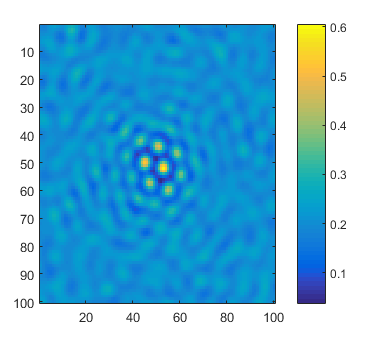
\includegraphics[width=0.5\textwidth]{fig_num/compareTestWavelet1}
}
\subfloat[]
{
    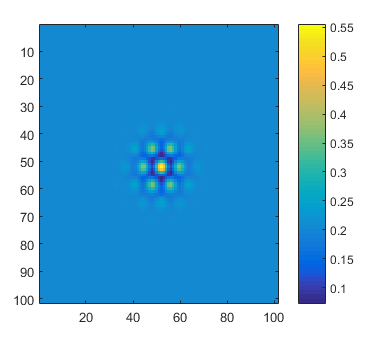
\includegraphics[width=0.5\textwidth]{fig_num/compareTestWavelet2}
}
\caption{(a) Solid grain surrounded by fluctuating liquid, observed in a simulation run with PFC model parameters $n_o=0.207$, $B^x=0.4$, $\Delta B=0.1650$, and $N_a=0.04$. (b) Constructed grain with same model parameters as (a) (except for fluctuations), and with chosen ratios $r_1=0.5$ and $r_2=0.8$. In both figures, the x-axis and y-axis are in number of grid points, and the color bar shows the value of the density field.}\label{fig:num_compareTestWavelet}
\end{figure}

As discussed in section \ref{sec:nuc_cnt_pfc}, we expect that critical nuclei in the PFC model will not depend on only the number of atoms as assumed by CNT. We thus develop a method to efficiently numerically approximate the form of critical nuclei in PFC under the slightly more flexible assumption that both size and order of a grain can vary during the nucleation process. We start by constructing a `test grain', whose density field is given by the predicted density field of a solid bulk in the one-mode approximation from equation \ref{eq:oneMode}, multiplied to a Gaussian envelope centered on one of the peaks. This is written as
%%
\begin{equation}\label{eq:num_testnuc}
n_{test}(x,y) = n_o + \phi \, e^{-(x^2+y^2)/2\sigma^2} \left(\frac{1}{2}\cos\left(\frac{4\pi}{\sqrt[]{3} a}y\right) - \cos\left(\frac{2\pi}{a}+\pi\right)\cos\left(\frac{2\pi}{\sqrt[]{3} a}y\right) \right)
\end{equation}
%%
where the average density of the system $n_o$ and the lattice constant $a$ depend on the model and its chosen parameters as usual, while $\phi$ and $\sigma$ are assumed to be the values that characterize a grain. We set $\phi=r_1 \phi_s$ where $\phi_s$ is the predicted amplitude in the solid bulk, given in equation \ref{eq:freeEnergy_minima}, and $r_1$ is a ratio between 0 and 1. Similarly, set $\sigma=r_2 \, a$ for some ratio $r_2>0$. Effectively, the ratio $r_1$ sets the relative order of the grain with respect to the original liquid and final solid phases, while $r_2$ determines the size of the grain. The ratio $r_1$ can also be heuristically understood as determining the average number of vacancies in the lattice of the forming grain, as it has been argued \cite{berry14} that variations in the amplitude of the PFC model's field can represent vacancy diffusion on diffusive time scales. Figure \ref{fig:num_compareTestWavelet} shows a grain that formed stochastically in a simulated PFC run, as well as a comparable grain constructed with equation \ref{eq:num_testnuc}. The work of formation for any constructed grain can be obtained by subtracting the energy of the unperturbed liquid phase given by equation \ref{eq:freeEnergy_minimized_liquid} from the energy of the grain's system calculated using equation \ref{eq:PFC_energyFunctional}. We note that this approximate grain construction is only expected to be valid for small-radius grains, as large stable solid grains would have a constant amplitude throughout their bulk and a finite interface width. Furthermore, this construction does not account for a variation in \textit{average density} of the grain's interior, as the constructed periodic field would average to $n_o$ over a large enough bulk.

For a given set of PFC model parameters and chosen $r_1$ and $r_2$, we can test whether the constructed grain of equation \ref{eq:num_testnuc} is post-critical or pre-critical by simulating it in a system consisting of the single grain in a much larger amount of liquid phase (grid size given by $L=512$). The fluctuation amplitude is set to zero in this simulation, as the grain is assumed to be the result of a prior fluctuation, and we are interested in the subsequent deterministic evolution of this grain. If after sufficient time steps the grain has grown to fill the system with solid, then it is known to be a post-critical grain, and vice versa. By repeating this test for various $r_1$ and $r_2$ (using a half-interval search method in one of the two variables, for efficiency), we obtain a curve in the space spanned by these two ratios that determines whether a grain with specific $r_1$ and $r_2$ is post-critical. Figure \ref{fig:num_ratioCurve} shows such a curve, which we will refer to as a `critical nucleus curve'. The form of the exactly critical nucleus is thus not unique, as any set of $r_1$ and $r_2$ lying on this curve would give a critical nucleus under the assumptions of the construction of equation \ref{eq:num_testnuc}.

\begin{figure}[!h]
\centering
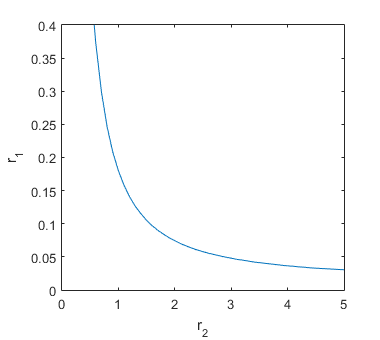
\includegraphics[width=0.6\textwidth]{fig_num/numRatioCurve.png}
\caption{The numerically determined critical nucleus curve for PFC parameters $n_o=0.207$, $B^x=0.4$, and $\Delta B=0.1650$. Choosing a set of ratios $r_1$ and $r_2$ lying above this curve results in a post-critical nucleus, and vice versa.}\label{fig:num_ratioCurve}
\end{figure}

%%%%%%%%%%%%%%%%%%%%%%%%%%%%%%%%%%%%%%%%%%%%%%%%%%%%%%%%%%%%%%%%%%%%%%%%%%%%%%%%%%%%
















\chapter{\sf Results}\label{ch:results}

This chapter presents the results of our numerical investigation into nucleation in the PFC model. We first present results for model parameters that follow the recommended noise amplitude given by the authors of \cite{kocher16}, as mentioned in section \ref{sec:pfc_dynamics}. We analyze these results in the presumed late-time asymptotic limit for which we obtained the CNT-predicted behavior of the nucleation rate and incubation time. We then use the numerical methods developed in sections \ref{sec:num_wave} and \ref{sec:num_testnuc} to examine the early formation shape and behavior of solid grains. Finally, we present further results under relaxed model parameter choice, to showcase nucleation dependence on noise amplitude.


%%%%%%%%%%%%%%%%%%%%%%%%%%%%%%%%%%%%%%%%%%%%%%%%%%%%%%%%%%%%%%%%%%%%%%%%%%%%%%%%%%%%
\section{Nucleation rates and incubation times}\label{sec:res_longtime}

A total of six data sets where obtained. Each data set consists of the averaged results of 50 to 150 simulation runs. All data sets had fixed PFC model parameters $n_o=0.207$, $B^x=0.4$, and $N_a=0.04$. The effective PFC temperature $\Delta B$ increases between the data sets, chosen to be $\Delta B=0.16500 + 0.00025\epsilon$ for $\epsilon$ an integer from 0 to 5 corresponding to the six sets in order from first to last. The noise amplitude $N_a$ was chosen within the recommended range corresponding to the other parameters as given in \cite{kocher16}, bearing in mind that these authors' results show that the variation range of $\Delta B$ between the data sets is too small to warrant a change in $N_a$ between the sets.

The parameters chosen for these runs place the simulated systems below their solidus (at $\Delta B \approx 0.1685$ for the chosen $n_o$ and $B^x$) on their phase diagram, and above their instability curves (at $\Delta B \approx 0.1642$). The range of $\Delta B$ was chosen such as to allow appreciable amounts of nucleation to take place in a reasonable amount of computational time, while remaining above the instability curve. We note that this range is small relative to the range between the instability curve and the solidus, and that the range lies closer to the instability curve than the solidus, indicating that the systems are greatly undercooled below their freezing point for nucleation to occur at noticeable rates. While this might be a result of making the PFC model's equations dimensionless, there is some precedence in physical systems for such homogeneous nucleation behavior. For example, in the absence of heterogeneous nucleation, water is known to remain liquid at temperatures of $235K$ and below \cite{mason58,jeffery97}. See also \cite{hoyt_phasetransf}, where an estimate for the variation of $J_{ss}$ with temperature is obtained using realistic values for an alloy. This estimate predicts that the homogeneous nucleation rate is undetectable before a specific temperature more than $100K$ below the alloy's freezing point, yet the rate rapidly increases beyond that specific undercooling temperature, similar to the behavior our results will show. Such undercooling behavior in alloys has also been observed experimentally \cite{provatas_coms2}.

Figure \ref{fig:res_I_datasets} plots the post-critical nuclei densities $I^*(t)$, corresponding to equation \ref{eq:nuc_crit_numdens}, for the first 5 sets. The sixth set, with $\epsilon=5$, is not visible on that figure's scale. We observe that the early portion of these curves resembles the form predicted by CNT, such as in figure \ref{fig:nuc_rates_fixedinc_b}, except that it is unclear whether the linearly increasing parts of these curves reach the true asymptote before tapering off to a constant value at late times due to the system fully transitioning to solid.

\begin{figure}[!h]
	\centering
	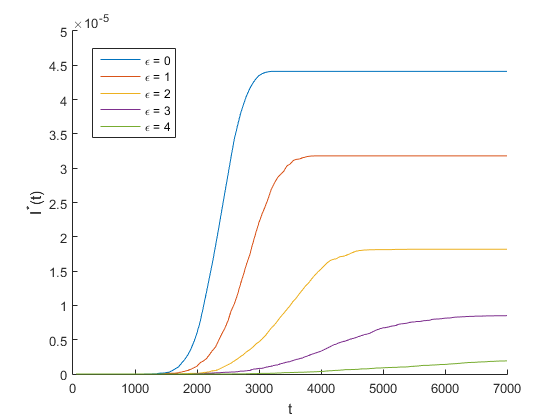
\includegraphics[width=0.7\textwidth]{fig_res/res_I_datasets}
	\caption{The post-critical nuclei densities for data sets $\epsilon=0$ to $\epsilon=4$.}\label{fig:res_I_datasets}
\end{figure}

\begin{figure}[!h]
	\centering
	\subfloat[]
	{
		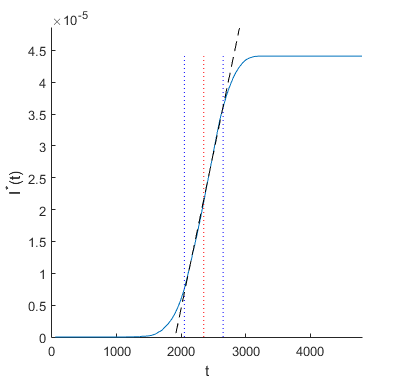
\includegraphics[width=0.5\textwidth]{fig_res/res_I0}
	}
	\subfloat[]
	{
		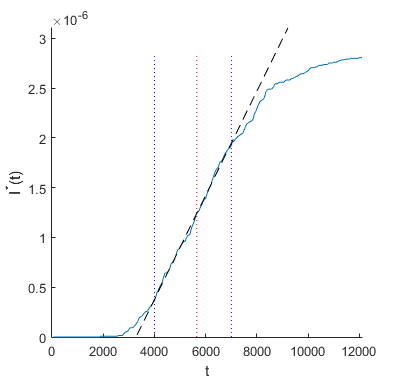
\includegraphics[width=0.5\textwidth]{fig_res/res_I4}
	}
	\caption{The geometric construction used to obtain $J_{ss}$ and $t^*$. The vertical blue dotted lines indicate the range of time taken to correspond to the asymptote. The dashed black line is the linear fit over that time range. Also shown as a vertical red dotted line is the time at which 10\% of the initial liquid volume has solidified. (a) Data set $\epsilon=0$, giving $J_{ss}=(4.9\pm 0.1)\times10^{-8}$ and $t^*=1910\pm 70$. (b) Data set $\epsilon=4$, giving $J_{ss}=(5.23\pm 0.08)\times10^{-10}$ and $t^*=3280\pm 90$. The errors on these values are from the uncertainty on the linear fit.}\label{fig:res_I_datasets_examples}
\end{figure}

We obtain the steady-state rate of nucleation $J_{ss}$ and the incubation time $t^*$ by the geometric construction described in section \ref{sec:nuc_fopl_sol}, taking as assumption that the linear part of each data set's $I^*(t)$ corresponds to the CNT-predicted asymptote. As a check for whether the assumption of asympoticity is sound, we also obtain for each data set the fraction of the initial liquid volume that has transitioned to solid as a function of time. We find that in all the data sets, only 10\% of the total liquid volume has solidified by the time approximately half of all nuclei have appeared. As the $I^*(t)$ curves have already entered the linear regime before that time, this suggests that the liquid has not yet been significantly depleted in the time range we assume to correspond to the asymptote. Figure \ref{fig:res_I_datasets_examples} demonstrates the geometric constructions for two of the data sets.%, as well as the time at which 10\% of the liquid volume has solidified.

\begin{figure}[!h]
	\centering
	\subfloat[]
	{
		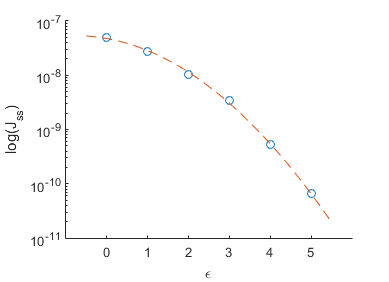
\includegraphics[width=0.5\textwidth]{fig_res/res_Jss_small}\label{fig:res_Jss}
	}
	\subfloat[]
	{
		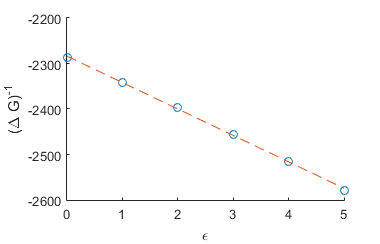
\includegraphics[width=0.5\textwidth]{fig_res/res_DG_tempdep_2}\label{fig:DG_tempdep}
	}
	\caption{(a) Plot of $J_{ss}$ for data sets $\epsilon=0$ to $\epsilon=5$ (blue circles), along with quadratic fit in semi-log space (red dashed line) showcasing faster than exponential decrease. Error bars are not visible at this scale. (b) Plot of $(\Delta G)^{-1}$ as a function of temperature $\Delta B$, over the range of temperatures for the data sets $\epsilon=0$ to $\epsilon=5$. Blue circles are calculated values, red dashed line is a linear fit.}
\end{figure}

Figures \ref{fig:res_Jss} plots $J_{ss}$ for the data sets, on a semi-log plot. Also shown is a quadratic fit in semi-log space to demonstrate faster than exponential decrease of $J_{ss}$ as effective temperature $\Delta B$ increases. To compare this change in rate to equation \ref{eq:nuc_Jss_scaling}, we only consider the effect of the exponential terms in that equation. As discussed in section \ref{sec:nuc_cnt_pfc}, we take $k_B T$ in the exponents to be constant as it depends on $N_a$, and $\Delta G_A$ and $\gamma$ to be positive and decreasing as $\Delta B$ increases. We must then turn to $\Delta G$ to explain the observed change in $J_{ss}$. Figure \ref{fig:DG_tempdep} plots $(\Delta G)^{-1}$ over the range of $\Delta B$ corresponding to the data sets, by estimating $\Delta G = F_s - F_l$ with the liquid and solid bulk energy densities obtained from section \ref{sec:pfc_phasediag}. We observe that this plot varies approximately linearly with $\Delta B$, meaning $\Delta G$ can only account for at most exponential decrease, not faster than exponential. This suggests either that the CNT definitions of $\Delta G$ and $\gamma$ are inadequate for the PFC model, as mentioned in section \ref{sec:nuc_cnt_pfc}, or that the linear fit in the geometric construction used to obtain $J_{ss}$ was not at the true asymptote, which might have resulted in a lower bound for $J_{ss}$ that is less accurate for the data sets of lower $\epsilon$.

We note that experimental predictions and results for physical materials do not disagree with the form of the $J_{ss}$ plot we obtained. Figure \ref{fig:res_Jss_examples} shows steady state homogeneous nucleation rates for water and a CuCo alloy, reproduced from experimental papers. We observe a faster than exponential decrease as temperature increases on the right parts of these plots. We are unable to access the equivalent of the left parts of these plots using the PFC model described in this work, as the decrease in nucleation rate as temperature decreases in these parts of the plots requires a model with a temperature-dependent solute mobility parameter.

\begin{figure}[!h]
	\centering
	\subfloat[]
	{
		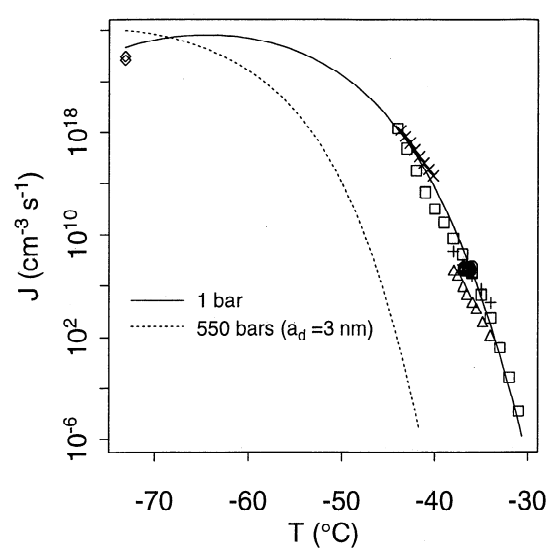
\includegraphics[width=0.5\textwidth]{fig_res/res_Jss_ex_water}
	}
	\subfloat[]
	{
		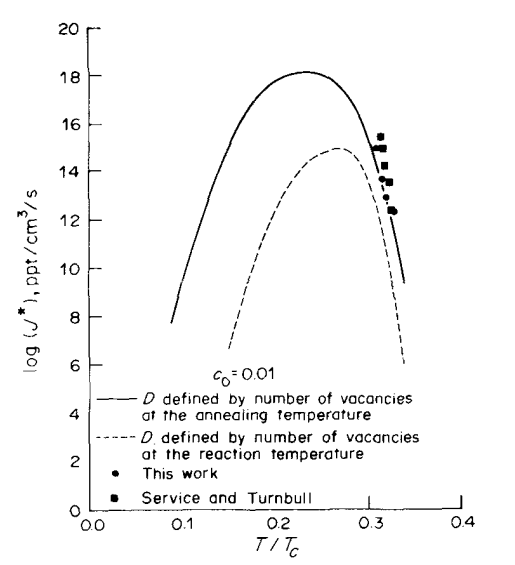
\includegraphics[width=0.5\textwidth]{fig_res/res_Jss_ex_cuco}
	}
	\caption{(a) Predicted steady state homogeneous nucleation rate for supercooled water, with some experimental results shown as symbols along the plot. Reproduced from \cite{jeffery97}. (b) Predicted steady state homogeneous nucleation rate for a CuCo alloy, with some experimental results shown as symbols along the plot. Reproduced from \cite{legoues84}.}\label{fig:res_Jss_examples}
\end{figure}

Figures \ref{fig:res_tinc} plots $t^*$ for the data sets. We observe that $t^*$ increases with temperature $\Delta B$. Comparing to equation \ref{eq:nuc_tinc_scaling}, the exponential term in that equation can not be the source of that increase under the assumptions that $k_B T$ depends on $N_a$ and $\Delta G_A$ decreases with one or both of the temperature parameters of the PFC model. As figures \ref{fig:res_I_datasets} and \ref{fig:res_I_datasets_examples} demonstrate that, for our datasets, the incubation time is larger than the time taken for $J^*(t)$ to increase from zero to $J_{ss}$, we can safely assume that $K>0$ in equation \ref{eq:nuc_tinc_scaling}. Recall that $\gamma$ in the PFC model decreases slowly with $\Delta B$. We take that $\gamma$ decreases much more slowly than $\Delta G$ increases, a fact that can be seen to hold due to the faster than exponential decrease of our calculated $J_{ss}$ despite a factor of $-\gamma^2/\Delta G$ in an exponential term in equation \ref{eq:nuc_Jss_scaling}. We can then conclude that the pre-exponential terms in equation \ref{eq:nuc_tinc_scaling} agree with an increase of $t^*$ with $\Delta B$ as observed, though no exact fit is attempted. This increase also agrees with the predictions for physical materials (for example, see the so-called TTT curves in \cite{legoues84}), again for temperatures where temperature-dependence of solute mobility is negligible.

\begin{figure}[h]
\centering
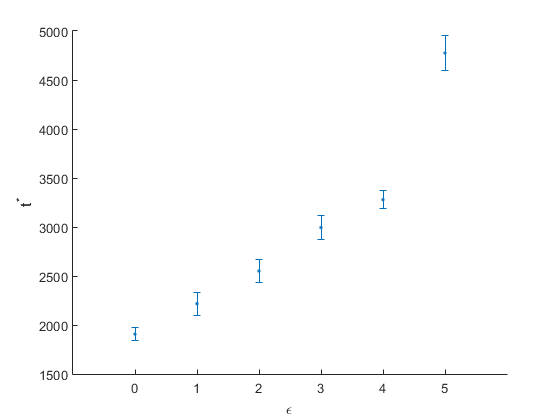
\includegraphics[width=0.8\textwidth]{fig_res/res_tinc}
\caption{Plot of $t^*$ for data sets $\epsilon=0$ to $\epsilon=5$.}\label{fig:res_tinc}
\end{figure}

%%%%%%%%%%%%%%%%%%%%%%%%%%%%%%%%%%%%%%%%%%%%%%%%%%%%%%%%%%%%%%%%%%%%%%%%%%%%%%%%%%%%
\section{Behavior of wave modes during nucleation}\label{sec:res_wavemodes}

In CNT, the stochastically appearing grains are assumed to form with the same lattice structure as the final solid phase. However, as the PFC model is based on a continuous density field, it is feasible that free-standing planar density waves or other non-lattice structures might temporarily appear in simulated PFC systems, especially during the early formation stages of solid grains. To assess whether such occurrences were prevalent in the simulation runs used to obtain the data sets of section \ref{sec:res_longtime}, we use the field filtering method developed in section \ref{sec:num_wave} to examine the growth of separate wave modes during the early formation of a few grains.

To obtain the relative amplitude growth of wave modes at points where nucleation events occur, the filtering process is applied every few time steps of a nucleation-rate simulation, for a range of rotation angles. The value of the filtered field at positions where nucleation occurs is then stored. Figure \ref{fig:res_wavelet_fieldvalues} plots the value of the filtered field at a specific point where nucleation was seen to occur, for a range of times and wavelet rotation angles, in a PFC system with model parameters corresponding to data set $\epsilon=4$. We see three peaks emerge, corresponding to the three wave modes expected in the final solid bulk. At the final time shown ($t=9000$), the post-critical nucleus is known to have grown to a size much larger than the critical size, indicating that the values of the field at that time is that of the final solid. We note that the height of the three peaks in the final solid are not equal as would be expected from the one-mode expansion of section \ref{sec:pfc_1mode}. This is assumed to be due to numerical error, as the square numerical grid has 4-fold symmetry while the final lattice structure has 6-fold symmetry, leading to slight numerical anisotropy in the application of the convolution filter.

 \begin{figure}[h]
	\centering
	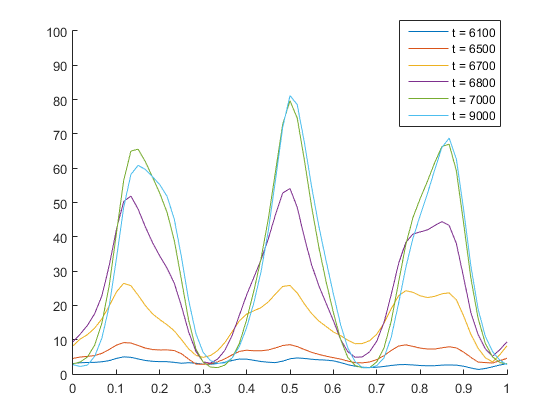
\includegraphics[width=0.7\textwidth]{fig_res/convField_byAngle}
	\caption{Value of the filtered field (y-axis) as a function of wavelet rotation angle (x-axis), for a range of times beginning before nucleation occurs and ending after the post-critical nucleus has grown to a size much larger than the critical size. The x-axis is in fractions of $\pi$.}\label{fig:res_wavelet_fieldvalues}
\end{figure}

Once the angles for the peaks of the filtered field are known at late times, we can plot the growth with time of the field for only these three angles starting from early times. Figure \ref{fig:res_convfield_nuc} plots the growth of these peaks for two nucleation events, with parameters corresponding to data set $\epsilon=0$. The values are normalized with respect to the maximum value attained by each peak, to account for the mentioned inequality of the peaks at late time due to numerical anisotropy. We also examined other nucleation events and obtained similar plots.


\begin{figure}[!h]
	\centering
	\subfloat[]
	{
		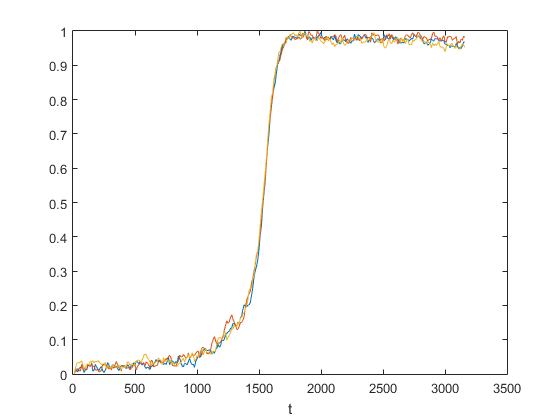
\includegraphics[width=0.47\textwidth]{fig_res/res_convfield_nuc_set20_event1}
	}\label{fig:res_convfield_nuc_a}
	\subfloat[]
	{
		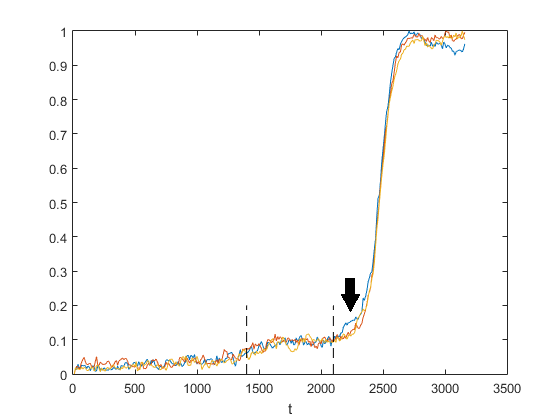
\includegraphics[width=0.47\textwidth]{fig_res/res_convfield_nuc_set20_event30_mod}\label{fig:res_convfield_nuc_b}
	}
	\caption{Normalized values of the filtered field at the angles where the three late time peaks are found (corresponding to the three shown colors), as a function of time, for two separate nucleation events in the same simulated system.}\label{fig:res_convfield_nuc}
\end{figure}

\begin{figure}[!h]
	\centering
	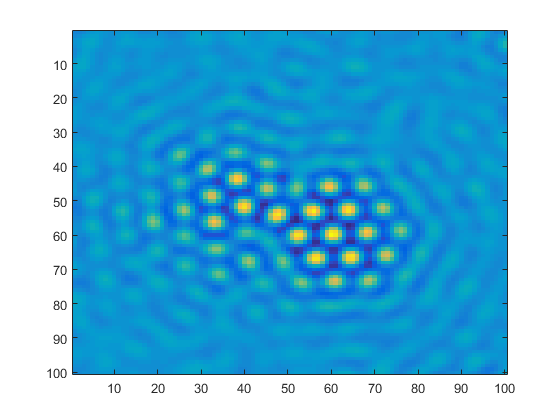
\includegraphics[width=0.6\textwidth]{fig_res/res_convfield_examplegrain}
	\caption{Density field of the grain from which peak filtered field values shown in figure \ref{fig:res_convfield_nuc_b} where obtained, at time $t=2550$. Axes indicate grid points.}\label{fig:res_convfield_examplegrain}
\end{figure}

The filtered field values at the three peak positions appear to vary in tandem during the majority of the process (up to the order of thermal fluctuations). This leads us to conclude that, at least for the parameter ranges of the data sets of section \ref{sec:res_longtime}, nucleation in the PFC model exhibits atomic lattice structure even during the relatively early parts of grain formation. However, a minority of examined grains display unexpected behavior of the field values at the three peaks, such as the grain corresponding to figure \ref{fig:res_convfield_nuc_b}. In that figure, the black arrow points to a relatively large fluctuation of only one mode that appears to precede the rapid growth of all three modes. The dashed lines denote a range of time where the three modes' growth seems to be delayed at a value higher than the background value, yet lower than the final solid value. We believe these behaviors are due to a few grains forming with more complex forms, unaccounted for in our assumptions. Figure \ref{fig:res_convfield_examplegrain} shows the grain corresponding to figure \ref{fig:res_convfield_nuc_b}. We observe that this grain appears to exhibit two separate lattice orientations. This is possibly due to it being formed from two grains that merged into one at an earlier time. Another possible explanation is the existence of a precursor non-crystalline phase or preferred structure that precedes criticality. The competition between these separate lattice orientations might explain the delay observed in \ref{fig:res_convfield_nuc_b}, as well as the single mode fluctuation before the final rapid growth.

These results indicate that the developed wave mode analysis method requires further refinement to be able to distinguish such edge cases. They also offer more insight into the difficulties involved in applying CNT to nucleation in the PFC model, as these complex-structured grains violate CNT's no-interaction or crystalline-structure assumptions, likely extending the required time for these grains to achieve criticality as their lattice structures stabilizes.






%%%%%%%%%%%%%%%%%%%%%%%%%%%%%%%%%%%%%%%%%%%%%%%%%%%%%%%%%%%%%%%%%%%%%%%%%%%%%%%%%%%%
\section{Critical nucleus curves for chosen parameters}\label{sec:res_testnuc}

We numerically calculate the `critical nucleus curves' for the parameters of data sets $\epsilon=0$ to $\epsilon=5$, using the method described in section \ref{sec:num_testnuc}. Figure \ref{fig:res_criticality} shows these curves. We observe that, as $\epsilon$ (equivalently, the effective temperature $\Delta B$) increases, the curves shift along both the relative order axis (y-axis) and size axis (x-axis). The shift along the size axis agrees with the basic prediction of CNT that critical radius must increase with temperature. However, CNT does not account for the shift along the order axis, as it assumes the lattice structure in the interior of the grain is always the same as that of the final solid. Further, the precise path that a forming grain would take through the $(r_1,r_2)$ parameter space before becoming a post-critical nucleus can not be predicted by CNT, instead requiring at least a 2 parameter theory similar to that developed in \cite{lutsko15} for the case of nucleation in globular protein systems. We expect that the most likely path to criticality will depend on a balance between statistically probable fluctuation amplitude and diminishing correlation at range: A critical nucleus of too small radius is unlikely to form due to the exponentially decreasing odds of obtaining a sufficiently large fluctuation as required field amplitude increases, while a critical nucleus of too large radius is unlikely to form before smaller grains because the spatially conserved density fluctuations in the system limit the rate at which mass and information of the forming lattice structure can propagate at large distances.

\begin{figure}[h]
	\centering
	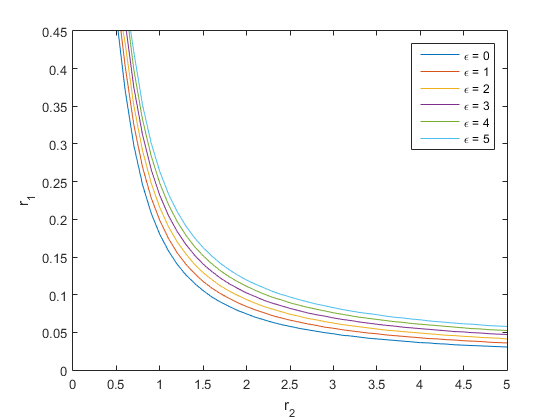
\includegraphics[width=0.8\textwidth]{fig_res/res_criticality}
	\caption{Critical nucleus curves for data sets $\epsilon=0$ to $\epsilon=5$. Recall that $r_1$ is a ratio that scales the amplitude of the density field of the grain, while $r_2$ scales the radius of the Gaussian-shaped grain.}\label{fig:res_criticality}
\end{figure}


%%%%%%%%%%%%%%%%%%%%%%%%%%%%%%%%%%%%%%%%%%%%%%%%%%%%%%%%%%%%%%%%%%%%%%%%%%%%%%%%%%%%
\section{Nucleation at different noise amplitudes}\label{sec:res_diffnoise}

The data sets of section \ref{sec:res_longtime} allowed the comparison of nucleation in the PFC model to CNT as the effective temperature $\Delta B$ varied. However, the chosen range of $\Delta B$ was too small to warrant a non-negligible change of $N_a$. It is of interest to examine the behavior of nucleation as a function of noise amplitude alone, to see whether our assumptions about the temperature dependence of the various values in equations \ref{eq:nuc_Jss_scaling} and \ref{eq:nuc_tinc_scaling} were warranted. In this section, we relax the requirement found by the authors of \cite{kocher16} on the noise amplitude parameter $N_a$, allowing it to be varied independently of $\Delta B$ over multiple new data sets. We stress that the new data sets' $J_{ss}$ and $t^*$ curves are not expected to vary as would be predicted for a physical system, as decoupling the choice of $N_a$ from $\Delta B$ effectively leads to the thermal fluctuations being unphysical.

We generate six new data sets with fixed model parameters $n_o=0.207$, $B^x=0.4$, and $\Delta B=0.1650$, and with increasing noise amplitude $N_a=0.030+0.002\kappa$ for $\kappa$ an integer from 0 to 5 corresponding to the six sets in order from first to last. Note that all these data sets would have the same critical nucleus curve as found for data set $\epsilon=0$ in section \ref{sec:res_testnuc}, since the critical nucleus curves depend on parameters $n_o$, $B^x$, and $\Delta B$, but not on $N_a$.

We repeat the procedure of section \ref{sec:res_longtime} for the new data sets. Figure \ref{fig:res_I_datasets_newnoise} plots their post-critical nuclei densities $I^*(t)$. Figure \ref{fig:res_I_datasets_examples_newnoise} demonstrates the geometric constructions for two of the data sets. Figures \ref{fig:res_Jss_newnoise} and \ref{fig:res_tinc_newnoise} plot $J_{ss}$ and $t^*$ for these data sets respectively. Note that the x-axes for these two plots are in terms of $T_r=N_a^2/2$, the fluctuation temperature obtained from the fluctuation-dissipation theorem as mentioned in section \ref{sec:pfc_dynamics}.


\begin{figure}[!h]
		\centering
	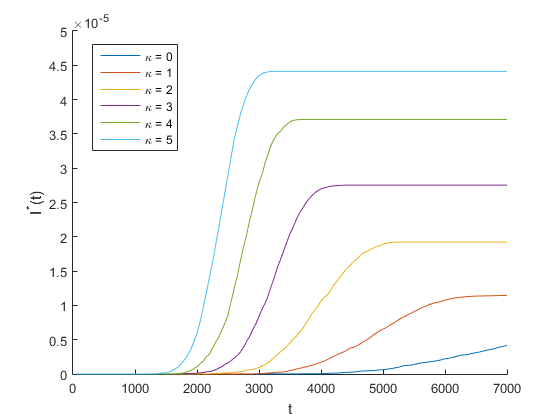
\includegraphics[width=0.7\textwidth]{fig_res/res_I_datasets_newnoise}
	\caption{The post-critical nuclei densities for data sets $\kappa=0$ to $\kappa=5$.}\label{fig:res_I_datasets_newnoise}
	\centering
	\subfloat[]
	{
		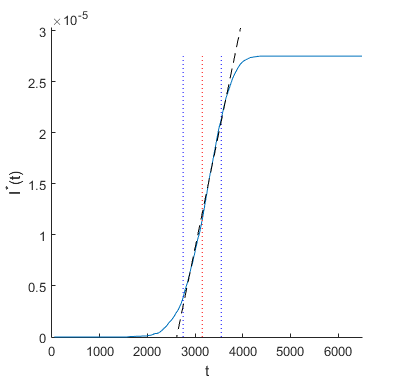
\includegraphics[width=0.5\textwidth]{fig_res/res_Ik2}
	}
	\subfloat[]
	{
		\includegraphics[width=0.5\textwidth]{fig_res/res_Ik5}
	}
	\caption{The geometric construction used to obtain $J_{ss}$ and $t^*$. The vertical blue dotted lines indicate the range of time taken to correspond to the asymptote. The dashed black line is the linear fit over that time range. Also shown as a vertical red dotted line is the time at which 10\% of the initial liquid volume has solidified. (a) Data set $\kappa=2$, giving $J_{ss}=(2.26\pm 0.09)\times10^{-8}$ and $t^*=2600\pm 200$. (b) Data set $\kappa=5$, giving $J_{ss}=1.84\pm 0.04)\times10^{-9}$ and $t^*=4800\pm 200$. The errors on these values are from the uncertainty on the linear fit.}\label{fig:res_I_datasets_examples_newnoise}
\end{figure}


Considering only the exponential terms of equation \ref{eq:nuc_Jss_scaling}, and recalling that $\gamma$ and $\Delta G$ only vary with $\Delta B$, the observed variation of $J_{ss}$ is expected to be due to $\Delta G_A$ and $k_B T$. Setting $k_B T = T_r$, we attempt a fit of form $A_1\exp(-A_2/T_r)$ where $A_1$ and $A_2$ are fit parameters to the plot of $J_{ss}$, as shown on figure \ref{fig:res_Jss_newnoise}. The fit suggests agreement between equation \ref{eq:nuc_Jss_scaling} and our results, assuming $\Delta G_A+\pi\gamma^2/(-\Delta G)$ varies slowly over the considered range of $T_r$.

As for incubation time, again due to $\gamma$ and $\Delta G$ not varying for these data sets, equation \ref{eq:nuc_tinc_scaling} indicates that $t^*$ would scale as $\exp(+\Delta G_A/k_B T)$ with $\Delta G_A$ decreasing with temperature and setting $k_B T = T_r$. Figure \ref{fig:res_tinc_newnoise} suggests agreement with equation \ref{eq:nuc_tinc_scaling}, though a specific fit was not attempted as the error bars allow both exponential as well as linear fits to be plausible.

\begin{figure}[h]
	\centering
	\includegraphics[width=0.8\textwidth]{fig_res/res_Jss_newnoise_Trfit}
	\caption{Plot of $J_{ss}$ for data sets $\kappa=0$ to $\kappa=5$ (blue circles), along with a fit of form $A_1\exp(-A_2/T_r)$ for fit parameters $A_1=5.57\times 10^{-6}$ and $A_2=0.0036$ (red dashed line). Error bars are not visible at this scale. }\label{fig:res_Jss_newnoise}
\end{figure}

\begin{figure}[h]
	\centering
	\includegraphics[width=0.8\textwidth]{fig_res/res_tinc_newnoise}
	\caption{Plot of $t^*$ for data sets $\kappa=0$ to $\kappa=5$.}\label{fig:res_tinc_newnoise}
\end{figure}



%%%%%%%%%%%%%%%%%%%%%%%%%%%%%%%%%%%%%%%%%%%%%%%%%%%%%%%%%%%%%%%%%%%%%%%%%%%%%%%%%%%%











\chapter{\sf Conclusion}\label{ch:conclusion}

The stated goals of this work were to examine nucleation in the PFC model and attempt a comparison with the predictions of CNT. We have shown that the PFC model follows the qualitative predictions of CNT. For temperature parameters fixed to ensure correct capillary fluctuations \cite{kocher16}, homogeneous nucleation was found to only occur at strong undercoolings. The rate of nucleation was observed to not be constant, instead taking a certain amount of time to achieve its steady state behavior. The steady state rate of nucleation was shown to decrease at least exponentially as temperature increased, while incubation time was shown to increase with temperature. All these behaviors were also argued to agree with experimental nucleation rate predictions and results, within the constraint of negligible temperature dependence of the solute mobility parameter.

To further examine nucleation dependence on PFC model parameters, we studied nucleation behavior with fluctuation amplitude decoupled from the effective temperature of the PFC model. While the results of this decoupling are not to be considered physically accurate, they showcased the CNT-predicted dependence of the steady state nucleation rate and incubation time on fluctuation amplitude. Despite the PFC model not including a direct equivalent of the CNT-assumed activation energy for atoms jumping through phase interfaces, the steady state nucleation rate was shown to vary with fluctuation amplitude following a dependence agreeing with that predicted for a thermally activated process. Similarly, the incubation time was seen to decrease as fluctuation amplitude increased, as expected in a system where propagation of mass and information is limited by the amplitude of spatially conserved density fluctuations. 

Our work also entailed studying the limitations of CNT as applied to PFC. We argued that the finite size of simulation systems, as well as inevitable interaction between forming solid grains, would possibly lead to deviations from CNT predictions. While our calculated post-critical nuclei densities appeared to achieve asymptotic behavior before the late tapering-off due to depletion of the liquid phase, it remains unclear whether the obtained values of nucleation rate and incubation time were noticeably affected by finite size effects. We also examined the wave mode amplitudes in pre-critical grains, observing that, despite lattice structure appearing early on in the process, a minority of nucleation events displayed more complicated formation behavior that might affect the validity of growth rate and non-interaction assumptions used in CNT.

We numerically calculated `criticality curves' to examine the approximate form of critical nuclei in the PFC model, under the assumption that both size and order of a grain are allowed to vary. These curves indicated that the CNT assumption of single-parameter form dependence is likely insufficient to consistently predict nucleation in PFC. We suggest that a multi-parameter theory should be attempted, similar to the work in \cite{lutsko15}. In the case of the PFC model, the parameters required might include some or all of the following: grain size, relative order compared to final solid state, local average density, and interface width.

In conclusion, this work lends credence to the PFC model's attempt to bridge the gap between atomistic and mesoscale methods, in so far as nucleation is involved. Although significant tuning of the model is likely required to achieve quantitative agreement with experimental results, the expected qualitative features appear naturally, in contrast to mesoscale models such as traditional phase field methods, and with greater numerical ease than with atomistic models such as MD. Future tasks related to this topic might include the aforementioned multi-parameter extension to CNT, as well as the study of nucleation in more complex variations of the PFC model, such as models with temperature-dependent solute mobility, greater number of accessible phases and atomic species, and more sophisticated numerical techniques (notably, the amplitude expansion method \cite{elder10,yeon10}).


%-mention briefly advantages of pfc over pf/md...?
%
%-rates scaling as CNT
%
%-activation energy for atomic jumps probably wrong
%
%-shape not quite as CNT, requires 3+ parameter version (lubtsko paper, though mention difficulties of assumptions therein!) including density, radius, order, interface width...
%
%-subtle difference between 2 temperature parameters in PFC
%
%-give heuristic explanation for change of t^* with fluctuation amplitude?
%
%-great care must be taken in reintroducing langevin fluctuations after the vibrational fluctuations have been averaged out when deriving from CDFT (though kocher paper's cutoff is a start)





%\appendix

%%%%%%%%%%%%%%%%%%%%%%%%%%%%%%%%%%%%%%%%%%%%%%%%%%% REFERENCES
\setlength{\parskip}{0cm}
\addcontentsline{toc}{chapter}{\protect\hspace{3.5ex}\sf References}
\setlength{\itemsep}{-20pt}
\setlength{\parskip}{4pt}

%\bibliographystyle{aip}
%\bibliographystyle{unsrt}
%\bibliographystyle{plain}

%\bibliography{ref}
\printbibliography

\end{document} 